\documentclass[12pt]{article}
\usepackage{setspace}
\usepackage{caption}
\usepackage{amsmath}
\usepackage{tabularx}
\usepackage{float}
\usepackage{graphicx}
\usepackage{hyperref}
\usepackage{marginnote}
\usepackage[most]{tcolorbox}
\usepackage[acronym]{glossaries}
\hypersetup{
    colorlinks=true, 
    linkcolor=blue, 
    filecolor=magenta,      
    urlcolor=cyan, 
    pdftitle={Stat Project}, 
    pdfpagemode=FullScreen, 
    }
\usepackage{subfigure}

\usepackage{fancyhdr, lastpage}
\pagestyle{fancy}
\fancyhfoffset[L]{0.5cm}
\lhead{Energy Economy}
\fancyhead[R]{\nouppercase{\leftmark}}
\cfoot{Page \thepage\ of \pageref{LastPage}}

\onehalfspacing
\author{ABSTRACT}

\date{ }
\usepackage[inner=2.5cm, outer=1.5cm, bottom=2cm]{geometry}

\usepackage[Glenn]{fncychap}
\newacronym{epc}{EPC}{Energy Performance Certificate}
\newacronym{imd}{IMD}{Index of Multiple Deprivation}
\newacronym{ols}{OLS}{Ordinary Least Squares}
\newacronym{ons}{ONS}{Office for National Statistics}
\newacronym{lsoa}{LSOA}{Lower Layer Super Output Areas}
\newacronym{gor}{GOR}{Government Offices for the Regions}
\newacronym{sap}{SAP}{Standard Assessment Procedure}
\newacronym{sse}{SSE}{Standard Square Error}

\newglossaryentry{price1}{
    name=price\_1, 
    description={The first sales transaction Price of the house}
}
\newglossaryentry{price2}{
    name=price\_2, 
    description={The second sales transaction Price of the house}
}
\newglossaryentry{imdg}
{		name=imd\_score, 
		 description={Index of multiple deprivation (IMD) rank (where 1 is most deprived) assigned to the property}
}\newglossaryentry{income}
{		name=income\_score, 
		 description={Income deprivation rank (where 1 is most deprived) assigned to the property}
}\newglossaryentry{emp}
{		name=emp\_score, 
		 description={Employment deprivation rank (where 1 is most deprived) assigned to the property}
}\newglossaryentry{educ}
{		name=educ\_score, 
		 description={Education skills and training deprivation rank (where 1 is most deprived) assigned to the property}
}\newglossaryentry{health}
{		name=health\_score, 
		 description={Health deprivation and disability rank (where 1 is most deprived) assigned to the property}
}\newglossaryentry{crime}
{		name=crime\_score, 
		 description={Crime rank (where 1 is most deprived) assigned to the property}
}\newglossaryentry{barrier}
{		name=barrier\_score, 
		 description={Barriers to housing and services rank (where 1 is most deprived) assigned to the property}
}\newglossaryentry{living}
{		name=living\_score, 
		 description={Living environment deprivation rank (where 1 is most deprived) assigned to the property}
}
\makeglossaries

\begin{document}
\setlength{\headheight}{14.49998pt}

\newpage

\maketitle

This is an attempt to replicate and enhance the analyses presented in the paper `Is there an Economic Case for Energy-Efficient Dwellings in the UK Private Rental Market?' by Franz Fuerst, Michel Haddad, Hassan Adad. This report provides a summary of the methods we used and the sources we used to complete this project.

\textbf{Keywords} - Energy efficiency; Hedonic model; Regression; Split incentive problem; Repeat sales index.
\newpage
\tableofcontents
\newpage
\section{Introduction}
The split incentive problem, or the lack of proper incentives to undertake energy efficiency measures, is one of the most pressing issues in the private rental sector. One party, the landlord, makes capital investments in energy efficiency and does not gain immediately, but the advantages are reaped by another, the tenant, who benefits from lower utility costs and greater thermal comfort. This affects landlords' investment decisions and creates a barrier to achieving improved energy efficiency. The key point of contention is whether the landlord can charge a higher rent for a dwelling that is more energy-efficient. ``Does improved house energy efficiency contribute to higher home sales prices?''

We address the topic in \autoref{sec:hed}. The hedonic regression model is used, in which the price of a property is separated into several components connected with its related attributes, and obtains estimates of the contributory value of each component. Implicit prices are estimated by linear regression.

In section 4, we relate the housing prices to the socio-economic environment of the area. In section 5, we address another important question `how does the sale prices of houses fluctuate with time in years?' We use the repeat sales method introduced by Bailey, Muth, and Nourse (1963). Lastly we put forward our entire summary in \autoref{sec:conc}.

\section{Data and descriptive statistics}
The data set contains information on dwellings from a large sample of real estates in the United Kingdom (n=4, 201). There are 43 variables altogether and can be categorised into four classes: Repeat sales transactions variables, \acrfull{epc} variables, \acrfull{imd} variables, Geographical location variables. The authors of the original publication also wrote the data article on this dataset. 
The data was gathered by them from a number of publically available sources and filtered to make it easier to analyse.
\begin{itemize}
    \item \textbf{Step 1}: The information on residences that have been sold at least twice were obtained from Her Majesty's Land Registry's online database, which had residential transaction values from 1995 to 2012. 
    \item \textbf{Step 2}: The \acrshort{epc} rating data was acquired from the Domestic Energy Performance Certificate Register online database and then combined with the dataset. 
    \item \textbf{Step 3}: The socioeconomic data was then added to the dataset established in the previous stage, and a random draw was performed to collect observations from hundreds of different neighbourhoods across England and Wales to provide a representative sample. 
\end{itemize}
We proceed to explain the variables and highlight the key features of data. In the dataset the 4201 houses are indexed by id running from 1 to 4201.
\subsection{Repeat sales transactions variables}
The variables price \_1 and \gls{price2} represent the first and second sales prices, respectively which were brought on date\_1 and date\_2 respectively. From these raw variables, two derived variables are formed ln\_price\_1, ln\_price\_2 are formed by taking their respective logarithms of \gls{price1} and \gls{price2}; days\_between\_sale represents the number of days between date\_1 and date\_2. Another variable denoted by perc\_change\_p2\_to\_p1, notes the percentage change of \gls{price1} and \gls{price2}.
The \autoref{table:desc} show a summary of the transactional variables.\footnote{The header described as \textbf{Normal} refers to the Shapiro-Francia normality test. The null hypothesis is that the data is normally distributed.The R function ShapiroFranciaTest() is being used to calculate the p-values.}
\begin{table}[H]
\resizebox{\columnwidth}{!}{\begin{tabular}{l l l l l l l l l l}
\hline
Variable & Mean & Median & Std.Dev & Skewnwss & Kurtosis & Smallest & Largest & Obs & Normal
\\
\hline
\gls{price1} & 120190.8638 & 100000 & 189750.5168 & 23.9595 & 689.7001 & 6000 & 5660000 & 4201 & 1.3e-80 \\
\gls{price2} & 154575.3033 & 120000 & 263755.4659 & 24.4936 & 706.5711 & 25000 & 7900000 & 4201 & 8.317e-82 \\
ln\_price\_1 & 11.4558 & 11.5129 & 0.6549 & -0.0051 & 1.645 & 8.6995 & 15.5489 & 4201 & 1.6227e-21 \\
ln\_price\_2 & 11.7524 & 11.6952 & 0.5217 & 1.1602 & 5.0146 & 10.1266 & 15.8824 & 4201 & 1.7283e-35 \\
perc\_change\_p2\_to\_p1 & 0.4986 & 0.2 & 0.8323 & 3.1254 & 19.9221 & -0.622 & 10.4167 & 4201 & 8.4553e-59
\\
days\_between\_sale & 2400.0838 & 2196 & 1236.9192 & 0.5589 & -0.3239 & 187 & 6156 & 4201 & 2.245e-28 \\
\hline
\end{tabular}}
\caption{Descriptive statistics of the transactional variables}
\label{table:desc}
\end{table}

\begin{figure}[H]
    \centering
    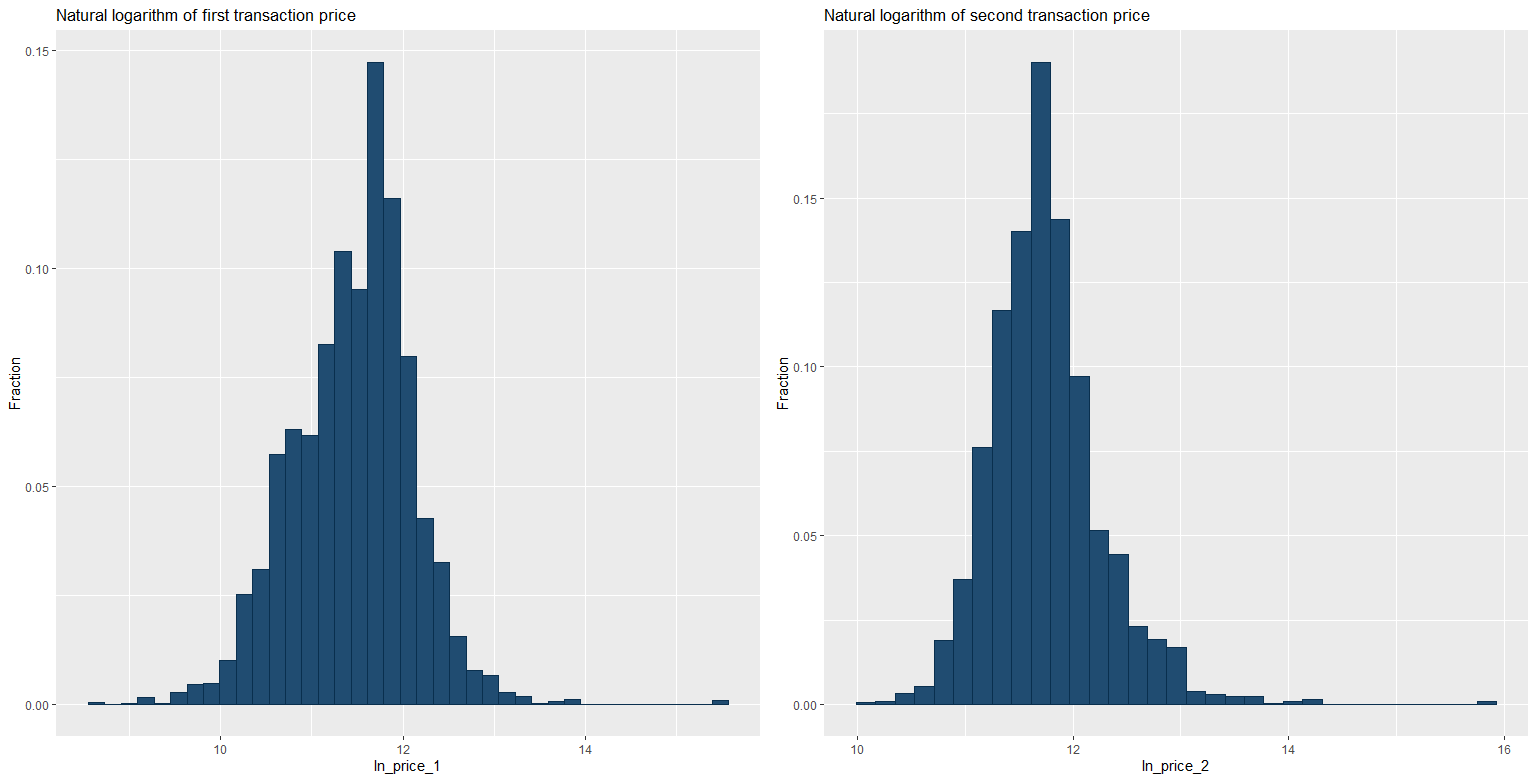
\includegraphics[width=15cm]{ln_price.png}
    \caption{Distributions of the log price paid in the first (upper left hand side) and second (upper right hand side) property sale transactions}
    \label{fig:transactional1}
\end{figure}

\begin{figure}[H]
    \centering
    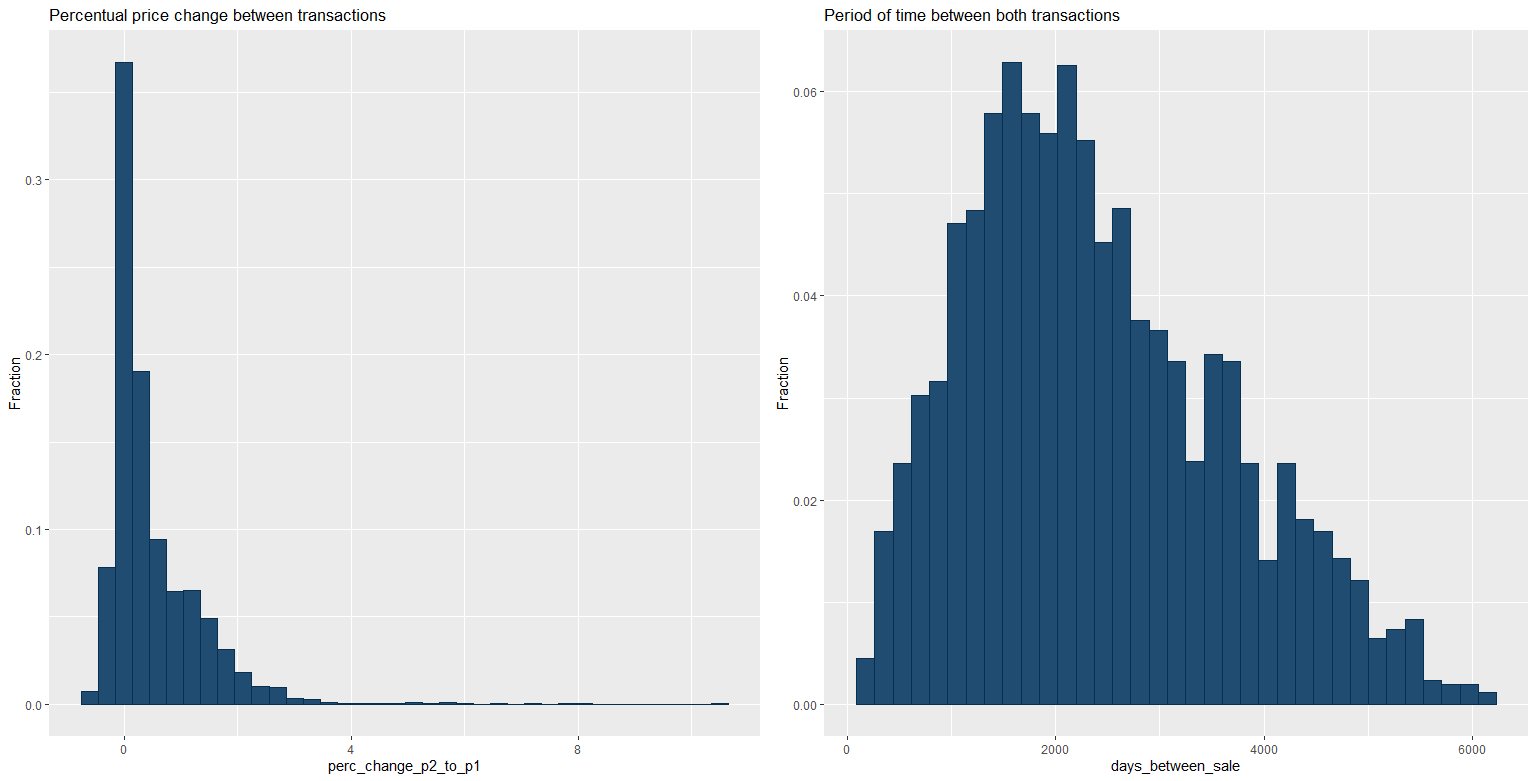
\includegraphics[width=17cm]{time_change.png}
    \caption{Price variation between the first and second sale transaction (left hand side), and period of time from the first to the second transaction (right hand side)}
    \label{fig:transactional2}
\end{figure}

\subsection{Energy performance certificate(EPC) variables}
An \acrshort{epc} is a rating system that describes the energy efficiency of real estate properties in the European Union. A score out of hundred denoted by epc\_100 is given to each house, where 1 is the least least efficient, and is based on \acrfull{sap} points. Each house was given an \acrshort{epc} band according to its \acrshort{epc} rating. A house belongs to a particular band in A, B, C, D, E, F, G if the \acrshort{sap} points is in the range of 92-100, 81-91, 69-80, 55-68, 39-54, 21-38, 1-20 respectively. The varaibles epc\_rating\_a, epc\_rating\_b, epc\_rating\_c, epc\_rating\_d, epc\_rating\_e, epc\_rating\_f, epc\_rating\_g are boolean variables which takes 1 if and only if the house is assigned to band A, B, C, D, E, F, G respectively. Another variable ln\_epc\_10 is obtained by taking logarithm of epc\_100. The \autoref{table:EPC} show the descriptive statistics of these variables. 

\begin{table}[H]
\centering
\begin{tabular}{c c c} 
 \hline
 EPC band & Frequency & Fraction \\ [0.5ex] 
 \hline
 EPC A & 0 & 0 \\ 
 EPC B & 379 & 0.0902\\
 EPC C & 1442 & 0.3433 \\
 EPC D & 1480 & 0.3523 \\
 EPC E & 699 & 0.1664 \\
 EPC F & 162 & 0.0386 \\
 EPC G & 39 & 0.0093 \\ [1ex] 
 \hline
\end{tabular}
\caption{Frequency and fraction of the seven \acrshort{epc} bands}
\label{table:EPC}
\end{table}


\begin{figure}[H]
    \centering
    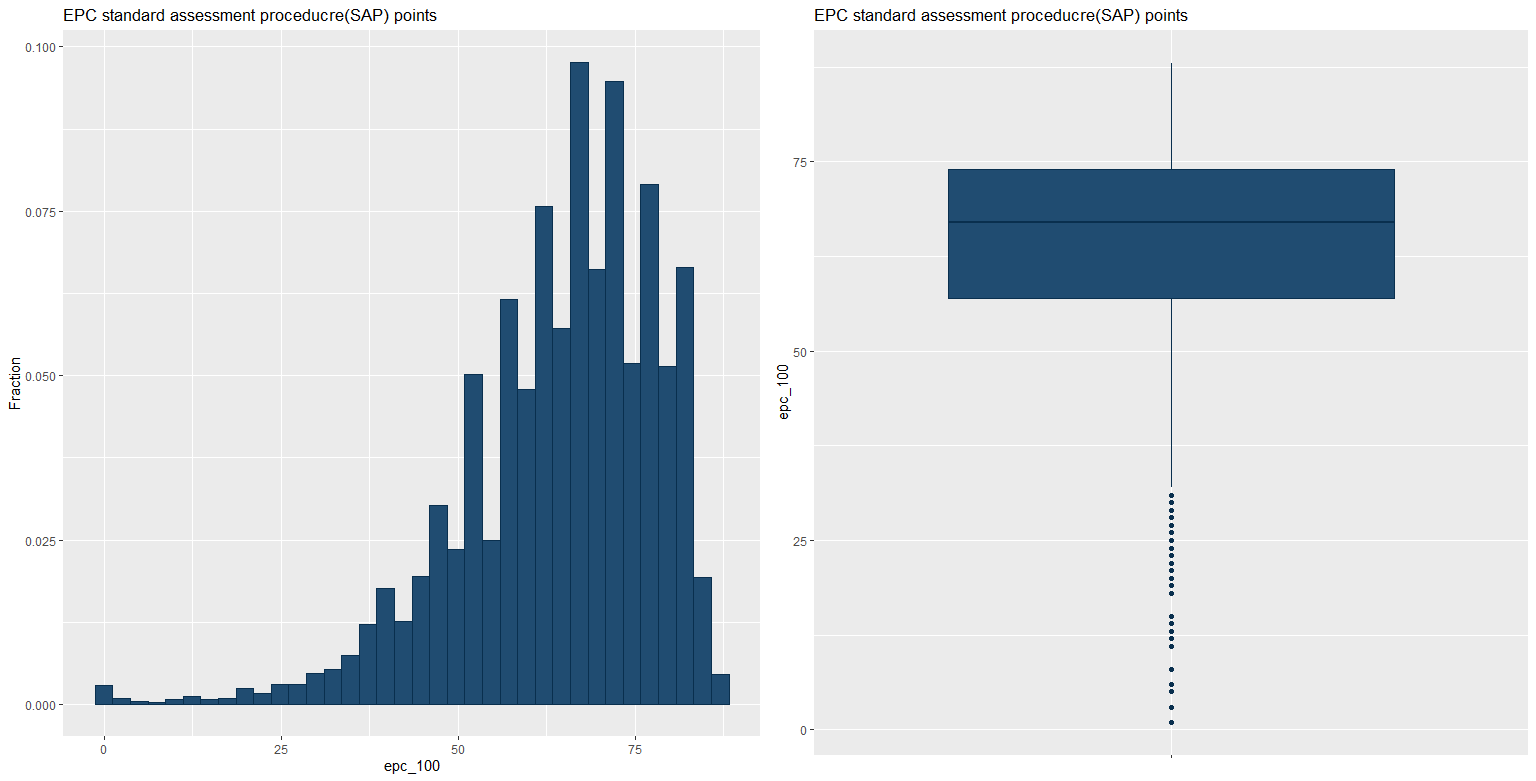
\includegraphics[width=17cm]{epc.png}
    \caption{Histogram (left hand side) and box plot (right hand side) of the distribution of the \acrshort{sap} points}
    \label{fig:EPCs}
\end{figure}

In this dataset, no property is assigned to band A. Most houses, around 70\%, have the rating C and D. Also, few data is available on \acrshort{epc} F and G. 
%Discussion needed

\subsection{Socio-Economic variables}
A rank is assigned to each of the \acrfull{lsoa} in the United Kingdom in terms of crime (\gls{crime}), education (\gls{educ}), income(\gls{income}) and employment (\gls{emp}), health (\gls{health}) and disability, barrier(\gls{barrier}), and living environment (\gls{living}). A rank indicating the level of deprivation (\gls{imdg}) is also given. In all these a rank of 1 is the most deprived. Each \acrshort{lsoa} is given score out of 1 to 10 in each of these criteria, where score 1 is the most deprived 10\% of \acrshort{lsoa}s. Thus we have the following categorical variables: imd\_level, income\_level, emp\_level, educ\_level, health\_level, crime\_level, barrier\_level, living\_level. 

\begin{figure}[H]
    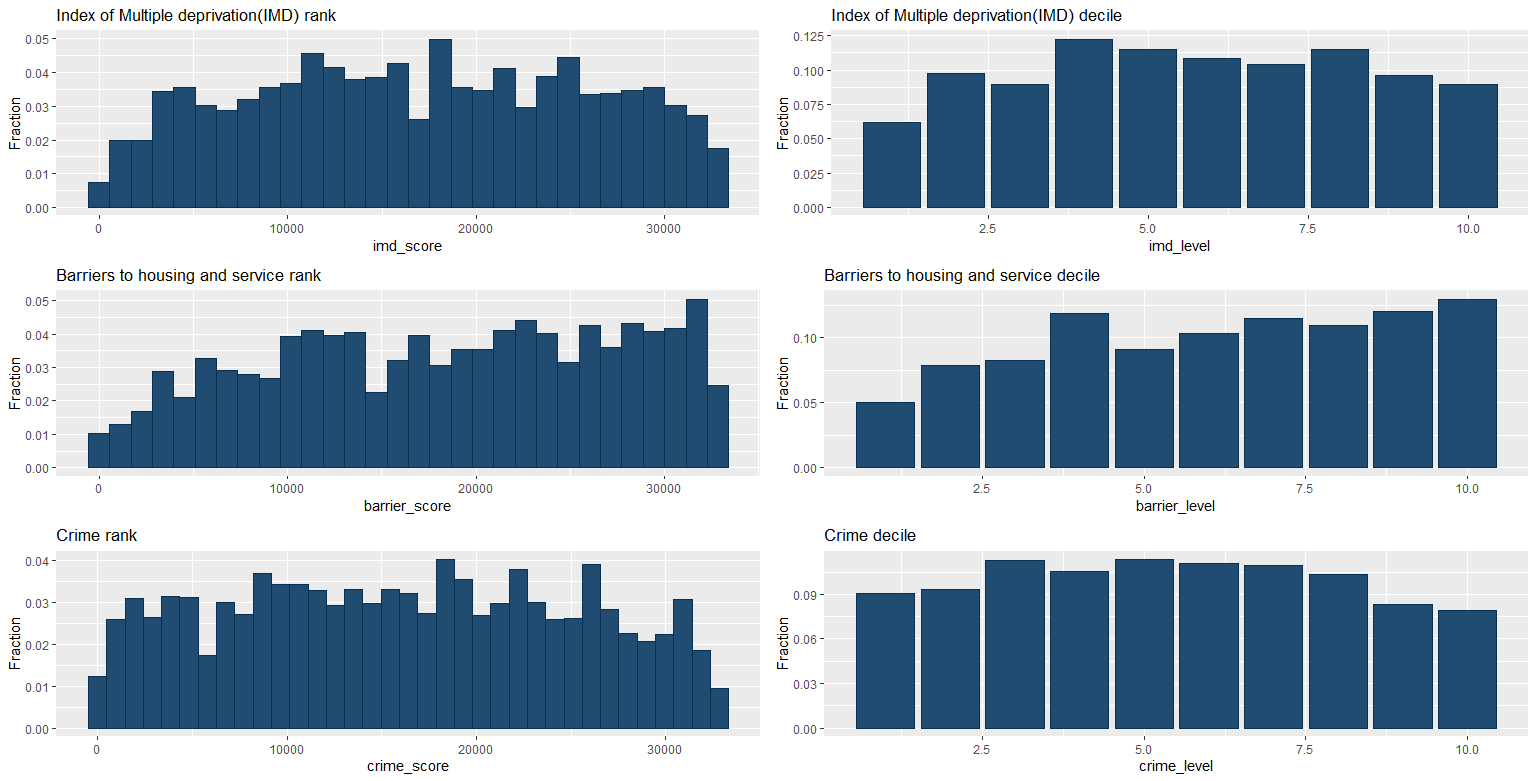
\includegraphics[width=18cm]{Rplot3.png}
    \caption{Histograms (left hand side) and bar charts (right hand side) of the \acrshort{imd} and its seven domains, considering their ranks and deciles, respectively}
    \label{fig:IMD1}
\end{figure}

\begin{figure}[H]
    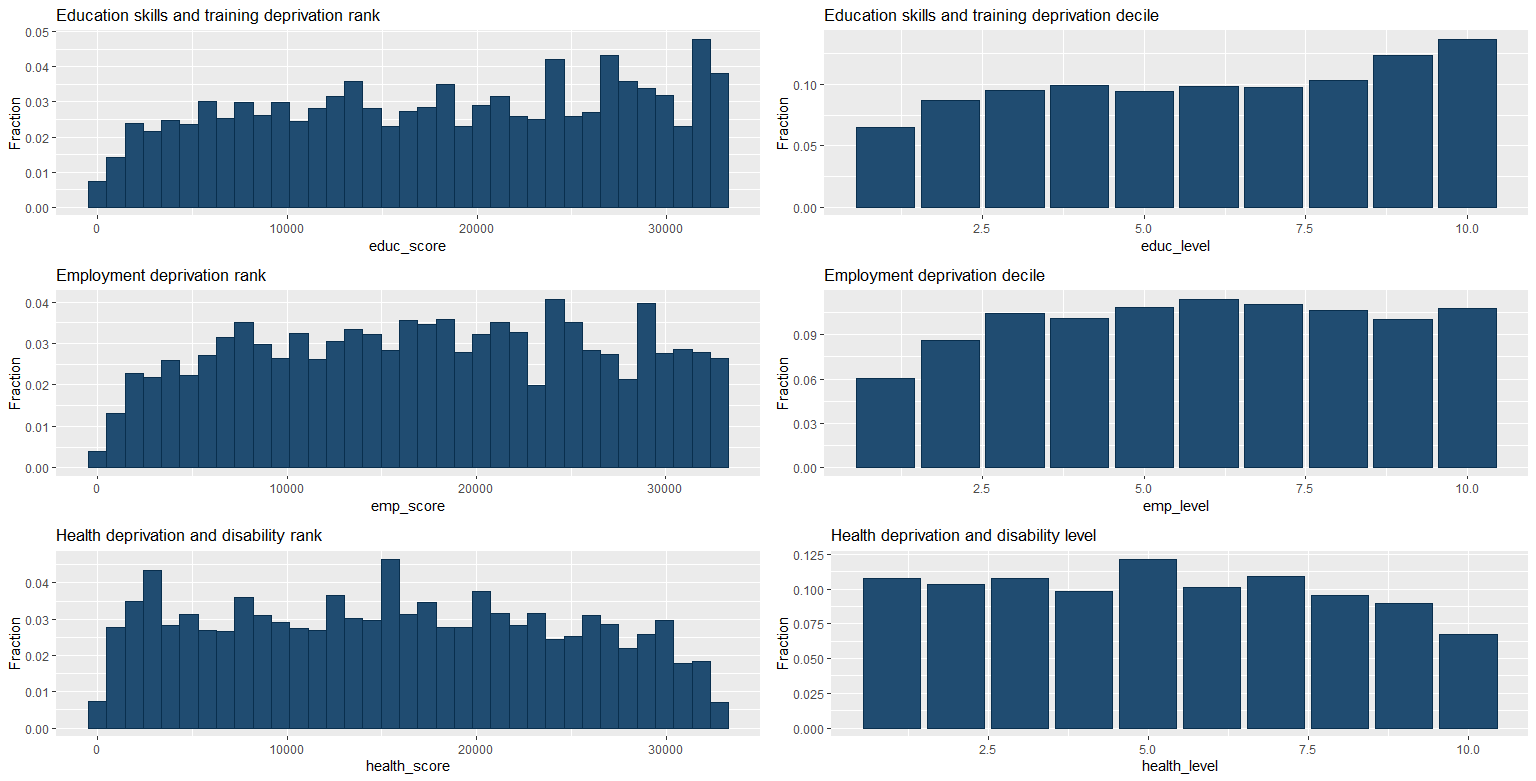
\includegraphics[width=18cm]{Rplot4.png}
    \caption{Continued}
    \label{fig:IMD2}
\end{figure}

\begin{figure}[H]
    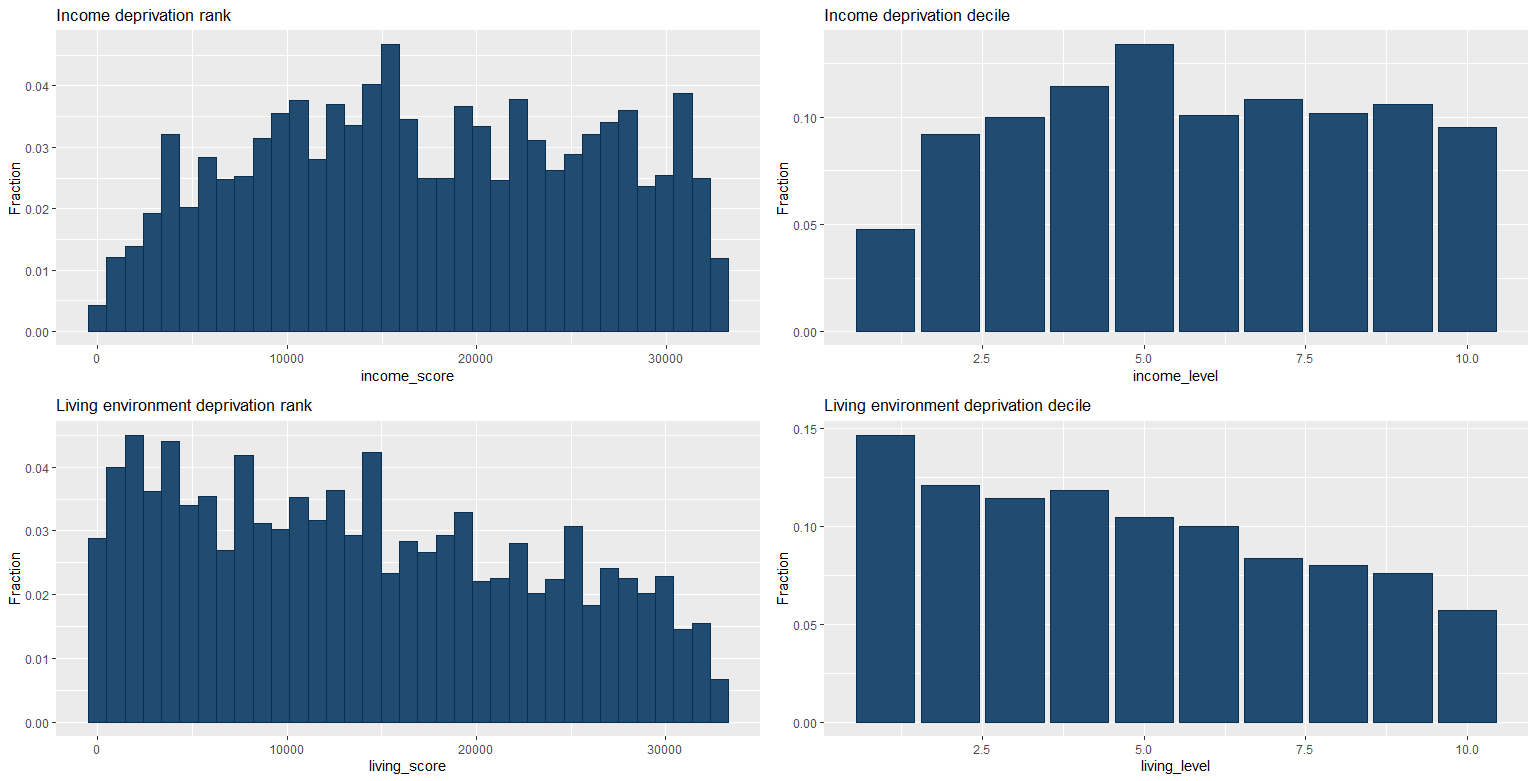
\includegraphics[width=18cm]{Rplot5.png}
    \caption{Continued}
    \label{fig:IMD3}
\end{figure}

\begin{figure}[H]
    \centering
    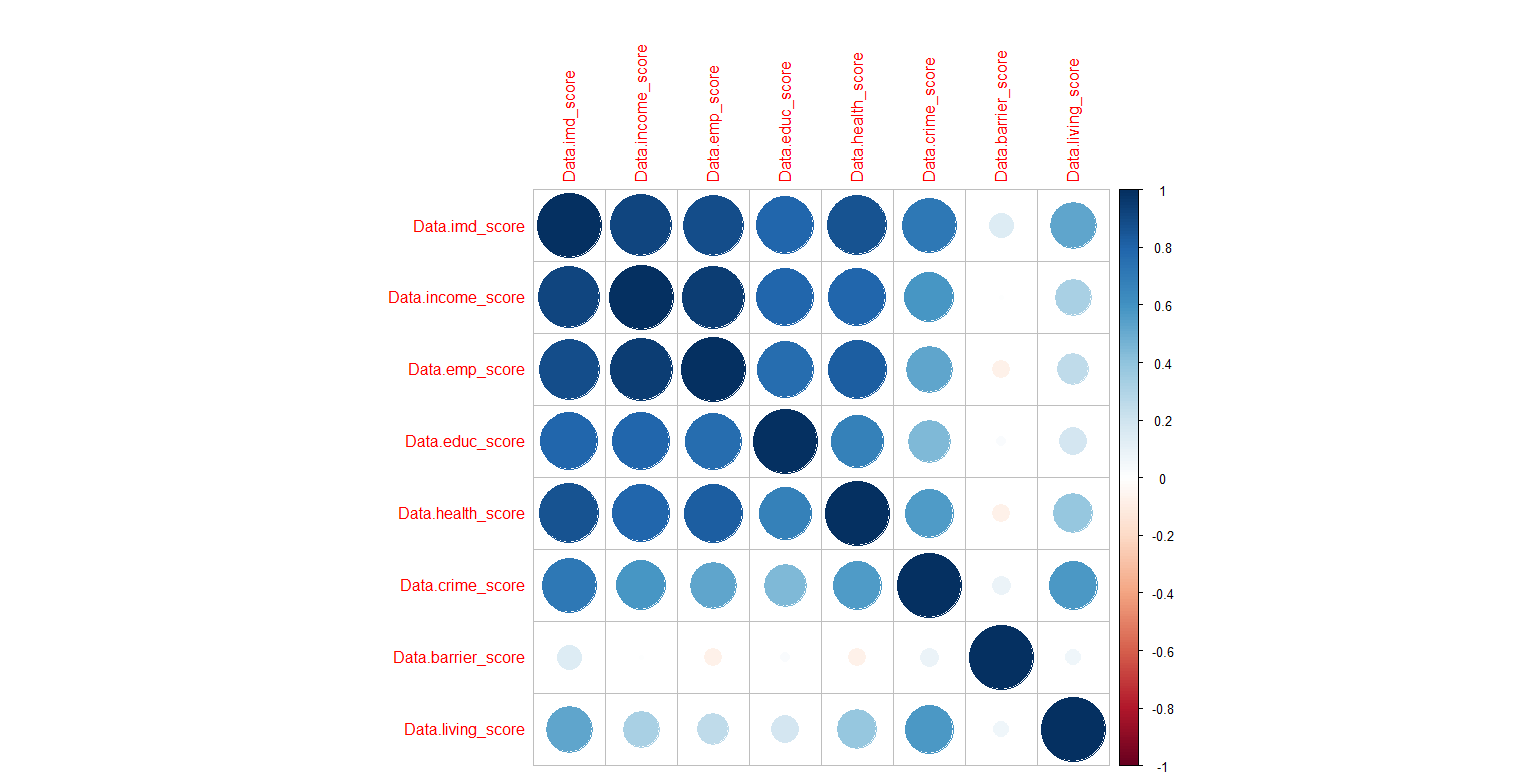
\includegraphics[width=18cm]{corrmat.png}
    \caption{Correlation matrix plot of socio-economic variables labelled according to the colors}
    \label{fig:corrmat}
\end{figure}

\subsection{Geographical location variables}
 The properties in dataset were distributed geographically according to the \acrfull{ons} categorization, which includes nine regions (previously known as \acrshort{gor}). The variables reg\_north\_east, reg\_north\_west, reg\_yorkshire\_and\_the\_humber, reg\_east\_midlands, reg\_west\_midlands, reg\_east\_of\_england, reg\_london, reg\_south\_east, reg\_south\_west are the boolean variables indicating the region in which property belongs to.

  \begin{table}[H]
\centering
\begin{tabular}{c c c} 
 \hline
 Geography & Transaction Frequency & Transaction fraction \\ [0.5ex] 
 \hline
 North West & 840 & 0.2 \\
 Yorkshire and the Humber & 839 & 0.1997 \\
 West Midlands & 599 & 0.1426 \\
 East Midlands & 435 & 0.1035 \\
 South East & 407 & 0.0969 \\
 London & 361 & 0.0859 \\
 South West & 287 & 0.0683 \\
 East of England & 279 & 0.0664 \\
 North East & 154 & 0.0367 \\ [1ex] 
 \hline
\end{tabular}
\caption{Geographical distribution of the transactions included in the dataset}
\label{table:geo}
\end{table}
 
 
\section{Hedonic pricing model and results}
\label{sec:hed}
Let $x_{i1t}, ..., x_{iKt}$ denote locational and physical characteristics, including categorical variables  related $i$th property. Let $P_{it}$ denote the price of $i$th property. As in the sample data we let $t=1, 2$. We make a probabilistic model as follows. The dependent variable $\ln (P_{it})$ is written as a linear function of $x_i$ and an error term $\varepsilon_i$ is added. 
$$\ln (P_{it})=\beta_{0t}+\sum_{j=1} ^{K} \beta_{jt}x_{ijt} +\varepsilon_i$$
The coefficients $\beta_{jt}$ are called hedonic price indices and are to be estimated.

The random errors capture additional information on the housing prices. We make four assumptions on the distribution of residuals $\varepsilon$ in the linear model:
\begin{itemize}
    \item The mean of $\varepsilon$ is 0
    \item The variance of $\varepsilon$ is $\sigma^2$
    \item $\varepsilon \sim N(0, \sigma^2)$
    \item The random errors are independent of each other.
\end{itemize}

The method of least square(\acrshort{ols}) is applied to find estimators $\hat \beta_{jt}$ of $\beta_{jt}$ and the estimated model is
$$\ln (\hat P_{t})=\hat \beta_{0t}+\sum_{j=1} ^{K} \hat \beta_{jt}x_{jt}$$
where $\hat P_{t}$ is the estimated sales price per square meter.
The coefficients $\hat \beta_{jt}$ can be interpreted as follows. Consider $x_{jt}$ for a particular $j$. If $x_{jt}$ is a numerical variable, then the above equation can be differentiated to yield 
$$\frac{\partial (\ln \hat P_{t})}{\partial x_{jt}}=\hat \beta_{jt}$$
$$\Rightarrow \frac{\partial \hat P_{t}}{\partial x_{jt}}=\hat \beta_{jt} \hat P_{t}$$

On the other hand if $x_{jt}$ is a categorical variable, hold all other variables constant and let $x_{jt}$ change to $x_{jt}+\Delta x_{ijt}$ and suppose $\hat P_t$ changes to $\hat P'_t$. Then, 
$$\ln(\hat P'_t)-\ln(\hat P_t)=\hat \beta_{jt}\Delta x_{jt}$$
$$\Rightarrow \hat P'_t=\hat P_t e^{\beta_{jt}\Delta x_{jt}}$$
Thus, for categorical variables, $e^{\hat \beta_{jt}}$ measures the prportion of change broght in the price for unit change in $x_{jt}$.

\subsection{Summary of important terms in regression}
\subsubsection{Multiple Regression Model}
Suppose we would like to predict variable $y$ using $x_1, \cdots, x_K$. We have the data:
$$y_i=\beta_0+\beta_1 x_{i1}+\cdots +\beta_n x_{iK}+\varepsilon_i={\textbf{x}_i^T\vec \beta}+\varepsilon_i$$

for $i=1, 2, ..., n$. 
Write 
$$X=\begin{bmatrix}
    1   & x_{11}       & x_{12} & x_{13} & \dots & x_{1K} \\
    1   & x_{21}       & x_{22} & x_{23} & \dots & x_{2K} \\
    \vdots   & \vdots & \vdots &\vdots &\vdots \\
    1 & x_{n1}       & x_{n2} & x_{n3} & \dots & x_{nK}
\end{bmatrix}, Y=\begin{bmatrix}
y_1\\
y_2\\
\vdots\\
y_n
\end{bmatrix}, \textrm{\textbf{e}}=\begin{bmatrix}
\varepsilon_1\\
\varepsilon_2\\
\vdots\\
\varepsilon_n
\end{bmatrix}$$
A model of the form
$\hat y=\hat \beta_0+\hat \beta_1 x_1+\cdots +\hat \beta_n x_K$
is to be fit to data, i.e. $\hat Y=X\hat \beta$. We need to find $\hat \beta $ that minimizes the \acrfull{sse}: $S(\hat \beta)=||Y-\hat Y||^2$.
\begin{itemize}
    \item Equate $\partial S/(\partial \hat \beta_i )=0$ and we obtain: $(X^T X) \hat \beta=X^T \textbf{Y}$.
    \item A formal solution is $\hat \beta=(X^T X)^{-1} X^T \textbf{Y}$. 
    \item The fitted values are $\hat Y=X\hat \beta=X(X^T X)^{-1}XY=H\textbf{Y}$ where $H$ is called the projection matrix.
    
    \item We make usual four assumptions on $\textrm{\textbf{e}}: E[\textbf{\textrm{e}}]=0, \textbf{\textrm{e}}~N_n(\vec 0, \sigma^2 I_K)$
    \item The covariance matrix of random vector $\hat \beta$ is $\Sigma_{\hat \beta \hat \beta}=\sigma^2 (X^T X)^{-1}$
\end{itemize}

The following is a summary of the important terms in the hedonic regression that will be used.
\subsubsection{Estimated coefficients} The \textit{Estimate} is the estimated coefficient by \acrshort{ols} regression. If the estimated coefficient is positive, then there is positive associativity between the corresponding variable and the price.
\subsubsection{Standard Error} \textit{Std.Error}: The standard error for each coefficient is given by
$$\sigma_{\hat \beta_{jt}}=\sigma^2[(X^TX)^{-1}]_{jj}$$
\subsubsection{Testing if a coefficient is zero} The testing of hypothesis whether a coefficient might be zero, using $t$-distribution is as follows.  We take the level of significance to be $0.01$.
    \begin{center}
        Null Hypothesis: $\beta_{jt}=0$
        
        Alternate Hypothesis: $\beta_{jt}\neq 0$
        
        test statistic: $t_c=\frac{\hat \beta_{jt}}{s_{\hat \beta_{jt}}}$
        
        Rejection region: $|t_c|>t_{\frac{0.01}{2}}$
        
        p-value: $2P(t>t_c)$ if $t_c$ is positive 
        
        and $2P(t<t_c)$ if $t_c$ is negative.
    \end{center} 
where the $t$-distribution has $n-(K+1)$ degrees of freedom.
\\ If we are 99\% confident that $\beta_{jt}\neq 0$, then we consider $x_{jt}$ to be a statistically significant in our model.
The p-value for this test is given in the last column. The significance code is given to each coefficient: , **, * indicate that the $p$-value is less than 0.001, 0.01, 0.05 respectively. The variables whose coefficients have , ** are statistically significant.
\subsubsection{{Residual standard error}} If $y$ is the dependent variable estimated by $\hat y$, the residual standard error $s$ is given by
$$s=\sqrt{\frac{SSE}{n-(K+1)}}=\sqrt{\frac{\sum {(y_i-\hat y_i)^2}}{n-(K+1)}}$$
$s$ is an unbiased estimator of $\sigma$.
\subsubsection{{Multiple R-squared}} If $y$ is the dependent variable estimated by $\hat y$, then the Multiple coefficient of determination $R$ is given by $$R^2=1-\frac{SSE}{SS_{yy}}=1-\frac{\sum {(y_i-\hat y_i)^2}}{\sum {(y_i- \overline{y}_i)^2}}$$ 
represents  the  proportion  of  the  total  sample  variation  in  $y$  that  can  be  ``explained'' by the multiple-regression model.
\subsubsection{{Adjust R-squared}} Adjust R-squared is defined as $$\overline{R} ^2=1-\frac{n-1}{n-(K+1)}(1-R^2)$$
The value of R may be large due to the excess number of regressors, which may not add to the regression's explanatory power. This is penalised by adjusted R-squared. 

\subsubsection{Confidence intervals for $\beta_{jt}$}
To each parameter $\beta_{jt}$, the 99\% ($\alpha = 0.01$) confidence interval using $t$-distribution is given by
$$(\hat \beta_{jt}-t_{\alpha/2}s_{\hat \beta_{jt}}, \hat \beta_{jt}+t_{\alpha/2}s_{\hat \beta_{jt}})$$
where $t_{\alpha/2}$ is the value such that, if $t$ has t-distribution of $n-(K+1)$ degrees of freedom, 
$$P(t>t_{\alpha/2})=\frac{\alpha}{2}$$
\subsection{Results of hedonic regression of prices}
Here are some preliminary plots before moving to regression. \autoref{fig:mprice} is the plot of mean of logarithm of prices plotted against the various \acrshort{epc} variables. As you can see here there are no \acrshort{epc} A because our dataset does not contain those variables.
\begin{figure}[H]
    \centering
    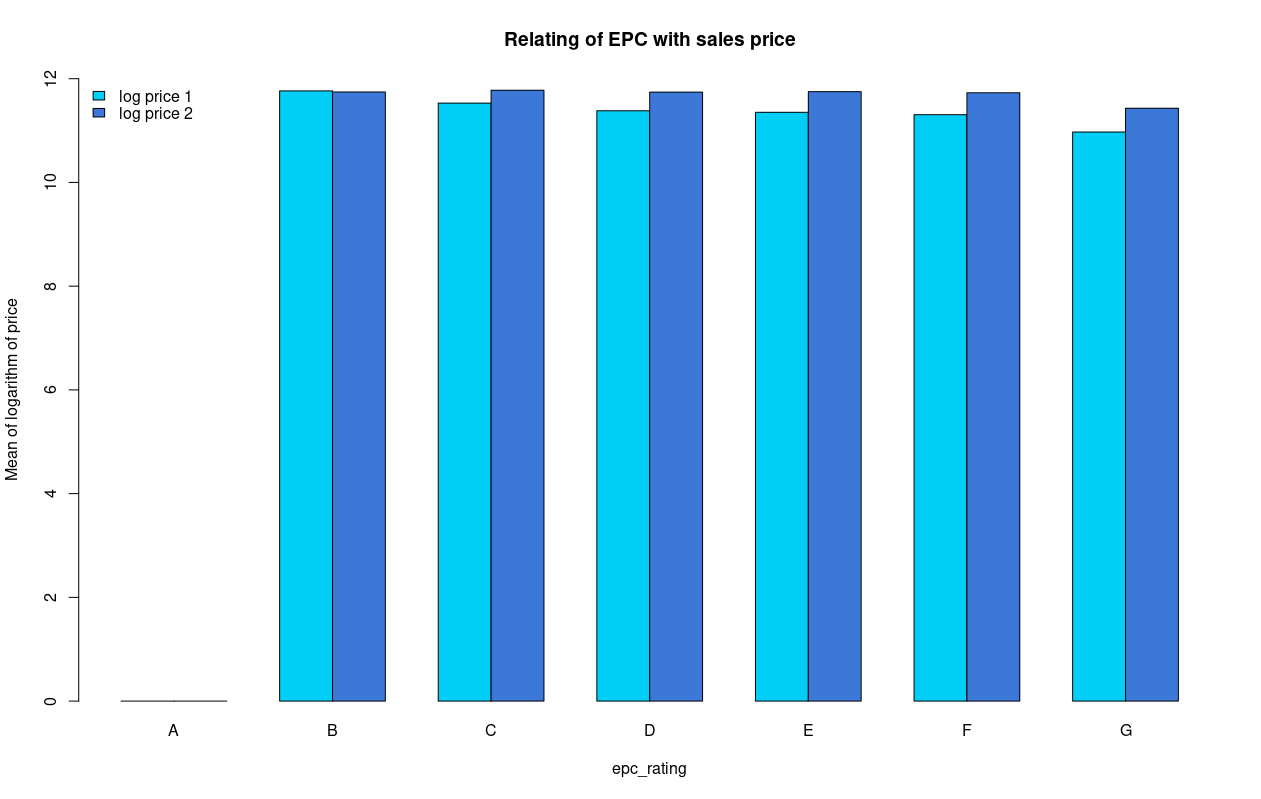
\includegraphics[width=12cm]{3.2. images/Rplot7.png}
    \caption{Plot of mean of ln\_price\_1 and ln\_price\_2 across different \acrshort{epc}s}
    \label{fig:mprice}
\end{figure}
In the \autoref{fig:boxprice}, the boxplot of ln prices again plotted against the different \acrshort{epc}s. This shows that there is a slight but some trend. In the x-axis 2 refers to \acrshort{epc} B, 3 to \acrshort{epc} C and so on. We can observe that there are many outliers captured by the boxplot. \acrshort{epc} C and D are neither the best nor the worst. Hence, there is a wide range of prices due to many investments on these categories. That is why there are so many outliers. On the other hand we can locate an outlier in B which is too far from the rest. That observation might be unusual. Furthermore, there is too less data on \acrshort{epc} G leading to less number of outliers.
\begin{figure}[H]
    \centering
    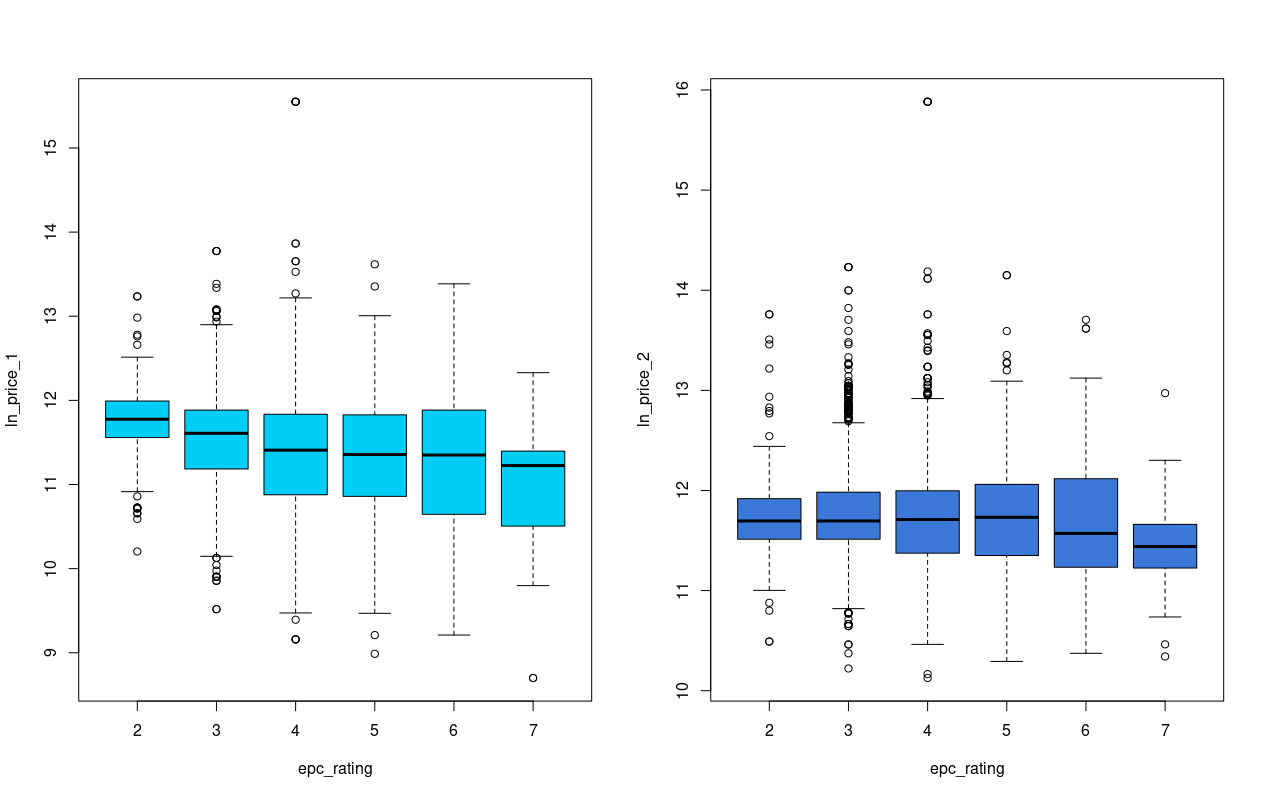
\includegraphics[width=16cm]{3.2. images/Rplot6.png}
    \caption{Box Plot for ln\_price\_1 and ln\_price\_2 respectively categorised by EPCs where 2:B, 3:C, 4:D, 5:E, 6:F, 7:G}
    \label{fig:boxprice}
\end{figure}
We have used R to estimate the hedonic pricing indices. The logarithm of prices was regressed on categorical variables epc\_rating\_b, epc\_rating\_c, epc\_rating\_e, epc\_rating\_f, epc\_rating\_g, and various regional indicators. As most houses have \acrshort{epc} rating D, epc\_rating\_d was taken as the baseline and is held out of the regression. epc\_rating\_a is removed as no houses in the sample has \acrshort{epc} rating A. reg\_north\_west is also taken as reference, as most houses in the sample are from this region. \autoref{table:1} and \autoref{table:2} shows the summary of this linear model. 

\begin{table}[H]
\centering
\begin{tabular}{c c c c c c} 
 \hline
 Variable & Estimate & Std Error & t-value & Pr($>|t|$) &  \\ [0.5ex] 
 \hline
 Intercept & 11.201346 &  0.024276 & 461.414 & 0(approx) & *** \\
 epc\_rating\_b & 0.412648 & 0.033911 & 12.168 & 0(approx) & *** \\
 epc\_rating\_c & 0.139870 & 0.021929 & 6.378 & $2\cdot 10^{-9}$ & *** \\
 epc\_rating\_e & -0.021471 & 0.027018 & -0.795 & 0.42684 &  \\   
 epc\_rating\_f & -0.103260 &  0.048702 & -2.120 & 0.03405 & * \\
 epc\_rating\_g & -0.371917 &  0.095488 & -3.895 & 0.00001 & *** \\
 reg\_north\_east & -0.002641 & 0.051658 & -0.051 & 0.95923 &  \\    
 reg\_yorkshire\_and\_the\_humber & 0.061126 &  0.028788 & 2.123 & 0.03378 & * \\
 reg\_east\_midlands & -0.002814 & 0.035063 & -0.080 & 0.93605 &  \\   
 reg\_west\_midlands & 0.101695 & 0.031686 & 3.209 & 0.00134 & ** \\
 reg\_east\_of\_england & 0.203688 & 0.040687 & 5.006 & 0.0000006 & *** \\
 reg\_london & 0.882822 & 0.037107 & 23.791 & 0(approx) & *** \\
 reg\_south\_east & 0.496382 & 0.035536 & 13.968 & 0(approx) & *** \\
 reg\_south\_west & 0.239821 & 0.040296 & 5.951 & $3\cdot 10^{-8}$ & *** \\ [1ex] 
 \hline
 \end{tabular}
 \caption{Hedonic regression of \gls{price1}. Signif. codes:  0 `***' 0.001 `**' 0.01 `*' 0.05 `.' 0.1 ` ' 1}
 \label{table:1}
 \end{table}

\begin{table}[H]
\centering
\begin{tabular}{c c c c c c} 
 \hline
 Variable & Estimate & Std Error & t-value & Pr($>|t|$) &  \\ [0.5ex] 
 \hline
  (Intercept) & 11.56700 & 0.01797 & 643.775 & 0(approx) & *** \\
 epc\_rating\_b & 0.03577 & 0.02510 & 1.425 & 0.15415 &  \\    
 epc\_rating\_c & 0.02668 & 0.01623 & 1.644 & 0.10026 &   \\  
 epc\_rating\_e & 0.02064 & 0.02000 & 1.032 & 0.30208 &  \\   
 epc\_rating\_f & -0.04066 & 0.03605 & -1.128 & 0.25942 &  \\   
 epc\_rating\_g & -0.27357 & 0.07067 & -3.871 & 0.00011 & *** \\
 reg\_north\_east & -0.06989 & 0.03823 & -1.828 & 0.06763 & . \\  
 reg\_yorkshire\_and\_the\_humber & 0.05109 & 0.02131 & 2.398 & 0.01653 & * \\  
 reg\_east\_midlands & -0.02497 & 0.02595 & -0.962 & 0.33599 &  \\   
 reg\_west\_midlands & 0.05897 & 0.02345 & 2.515 & 0.01195 & * \\
 reg\_east\_of\_england & 0.19067 & 0.03011 & 6.332 & 0(approx) & *** \\
 reg\_london & 0.98121 & 0.02746 & 35.727 & 0(approx) & *** \\
 reg\_south\_east & 0.47361 & 0.02630 & 18.007 & 0(approx) & *** \\
 reg\_south\_west & 0.25482 & 0.02982 & 8.544 & 0(approx) & *** \\ [1ex]
 \hline
\end{tabular}
\caption{Hedonic regression of \gls{price2}. Signif. codes:  0 `***' 0.001 `**' 0.01 `*' 0.05 `.' 0.1 ` ' 1}
\label{table:2}
\end{table}
 

\begin{figure}[H]
    \centering
    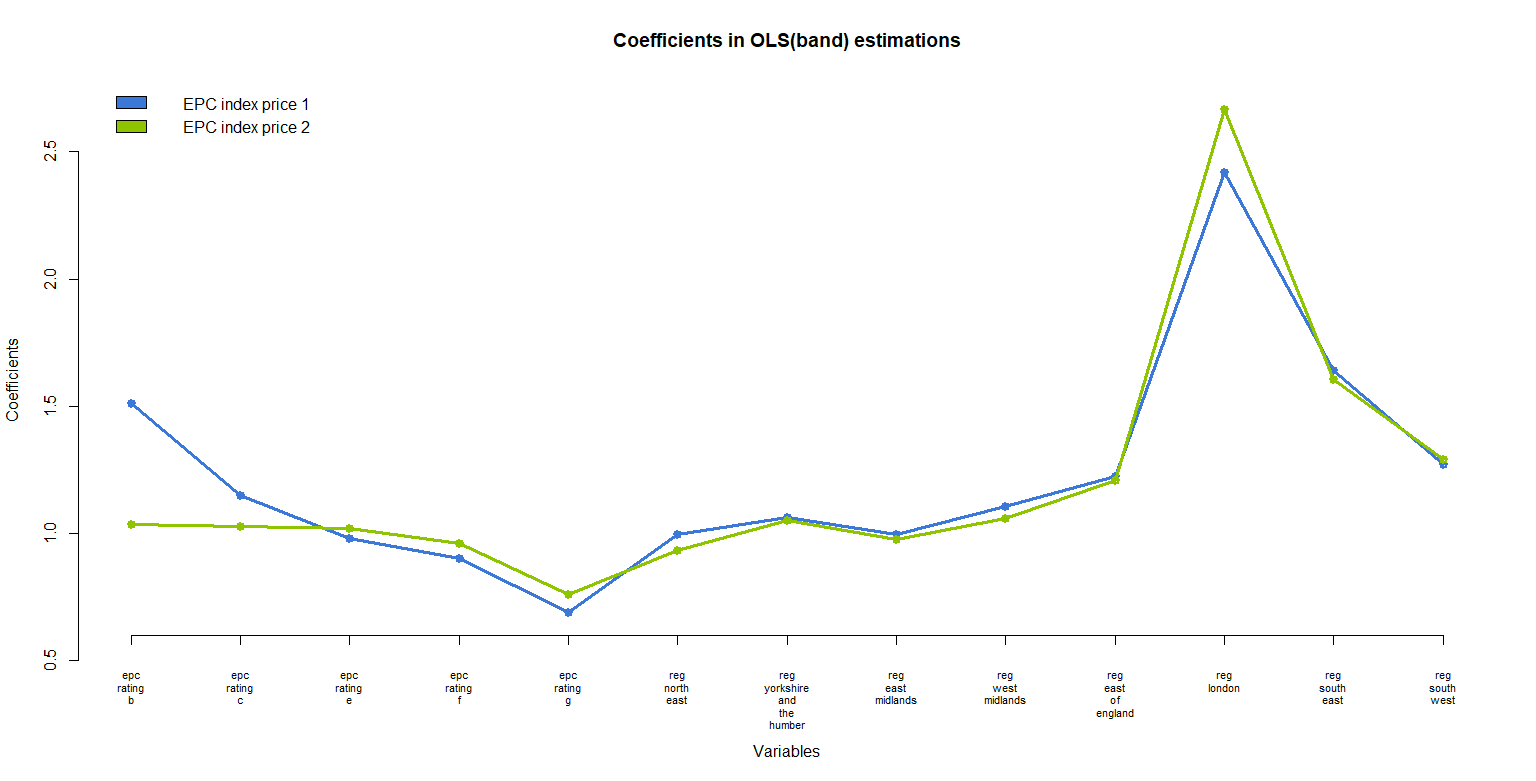
\includegraphics[width=18cm]{3.2. images/3.2linegraph_index.png}
    \caption{Hedonic Index of variables indicating the exponents of the regression coefficients}
    \label{fig:hedonic}
\end{figure}

The exponent of coefficients can be plotted on a line graph and is shown in above \autoref{fig:hedonic}. This shows the relation between  \acrshort{epc} rating and prices. From the \autoref{table:1}, we see that the epc\_rating\_b, epc\_rating\_c are statistically significant variables in this model. For \gls{price1}, epc\_rating\_b has hedonic index around 1.5, indicating that houses with \acrshort{epc} rating B experience a price premium. The hedonic index of epc\_rating\_g is less than 1, indicating that lower energy efficient homes tend to have lower prices. Region London has the highest hedonic index indicating that, with respect to houses in northwest region, houses in London are expensive.

\subsection{Diagnostic plots}
\label{diag_plot}
Residual is nothing but the difference between fitted values and true values. $$\varepsilon_i=y_i-\hat y_i$$ We made four assumptions on the distribution of these residuals in the beginning and now we diagnose if these assumptions hold, and assess if the model explains the relationship well.
\subsubsection{Residuals vs. Fitted}
This is a scatter plot of fitted values on x-axis and residual=true value$-$fitted values. These graphs indicate if the price and energy performance have a non-linear connection.
If the model does not capture the non-linear connection between predictor factors and outcome variables, the pattern may appear non-linear

%Two Figures 
\begin{figure}[H]
    \centering
    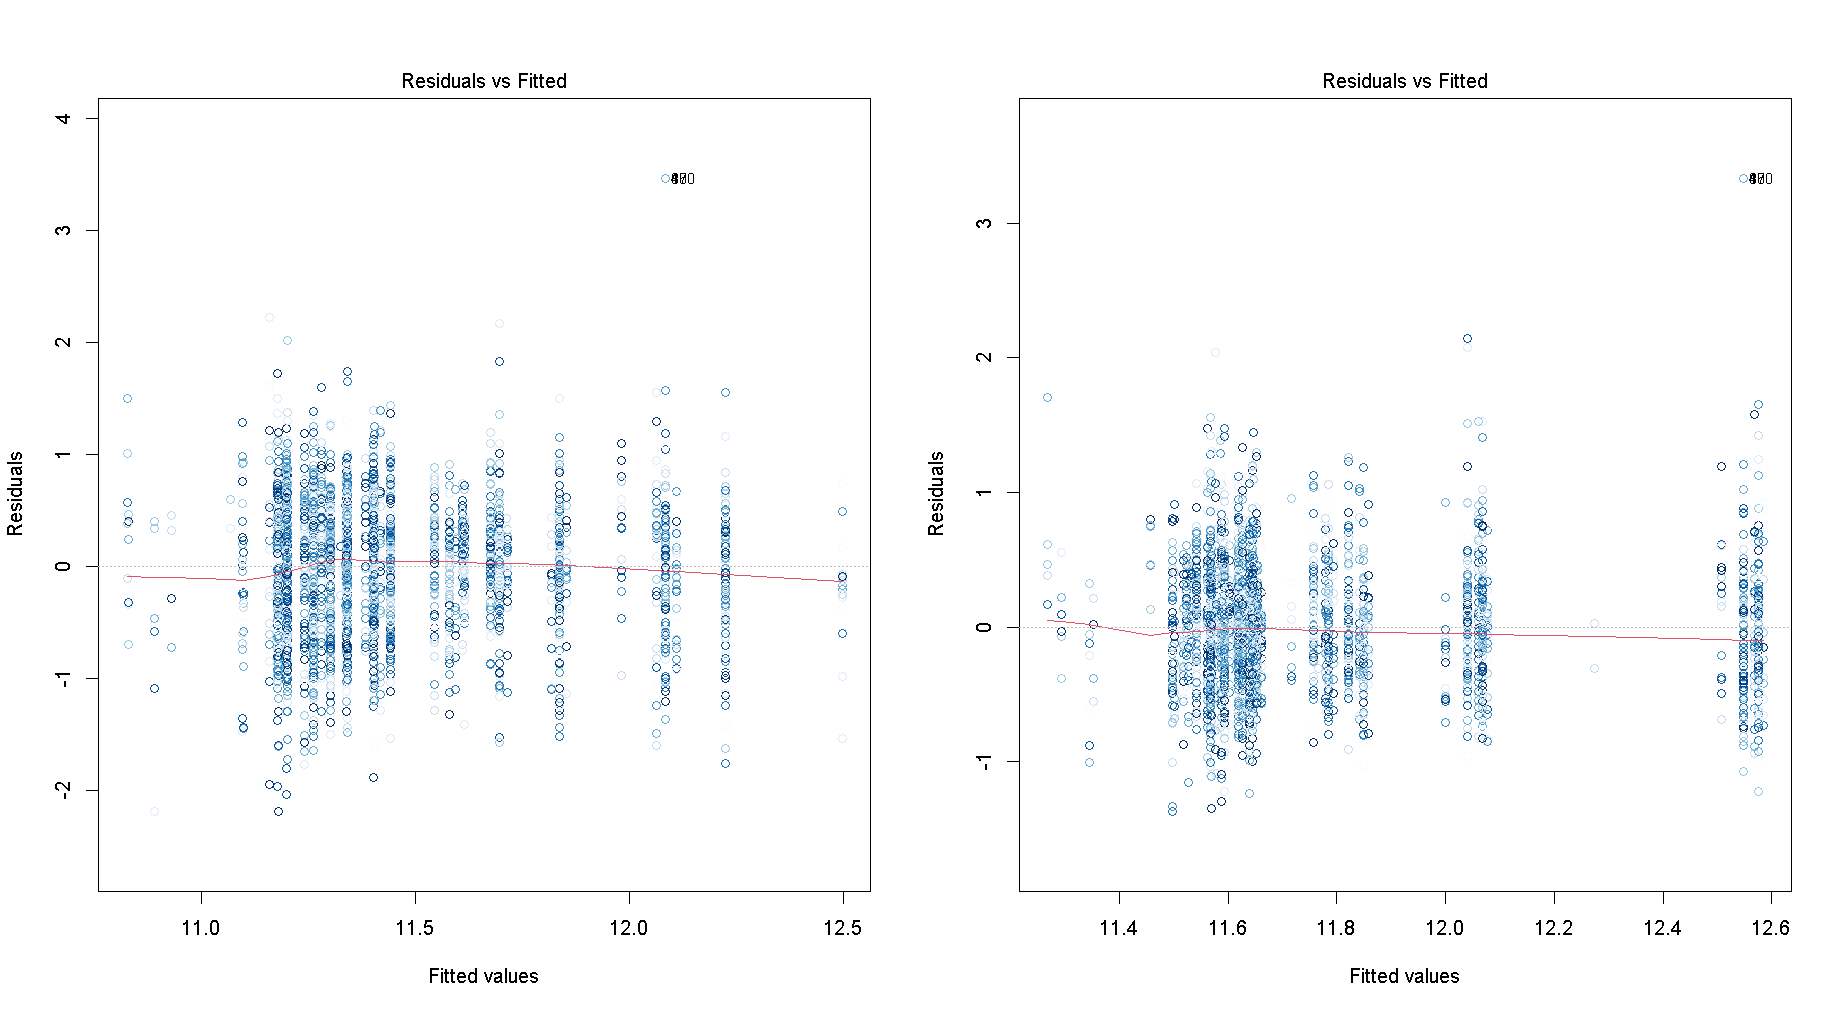
\includegraphics[width=18cm]{3.3 images/3.3.1plot.png}
    \caption{Plot of Residuals vs Fitted}
    \label{fig:residue}
\end{figure}

Fig shows the residuals versus fitted plot for the two models. Both the graphs show that the relationship between prices and locational factors, energy performance is nearly linear and our model explains this relationship quite well.

\subsubsection{Normal Q-Q plots of residuals}
This is a scatter plot with theoretical normal quantiles on x-axis and quantiles of residues in y-axis. This plot diagnoses if the residuals are normally distributed. The figures below show that the residuals in this model are almost normally distributed, in accordance with our assumptions.

%Two Figures 

\begin{figure}[H]
    \centering
    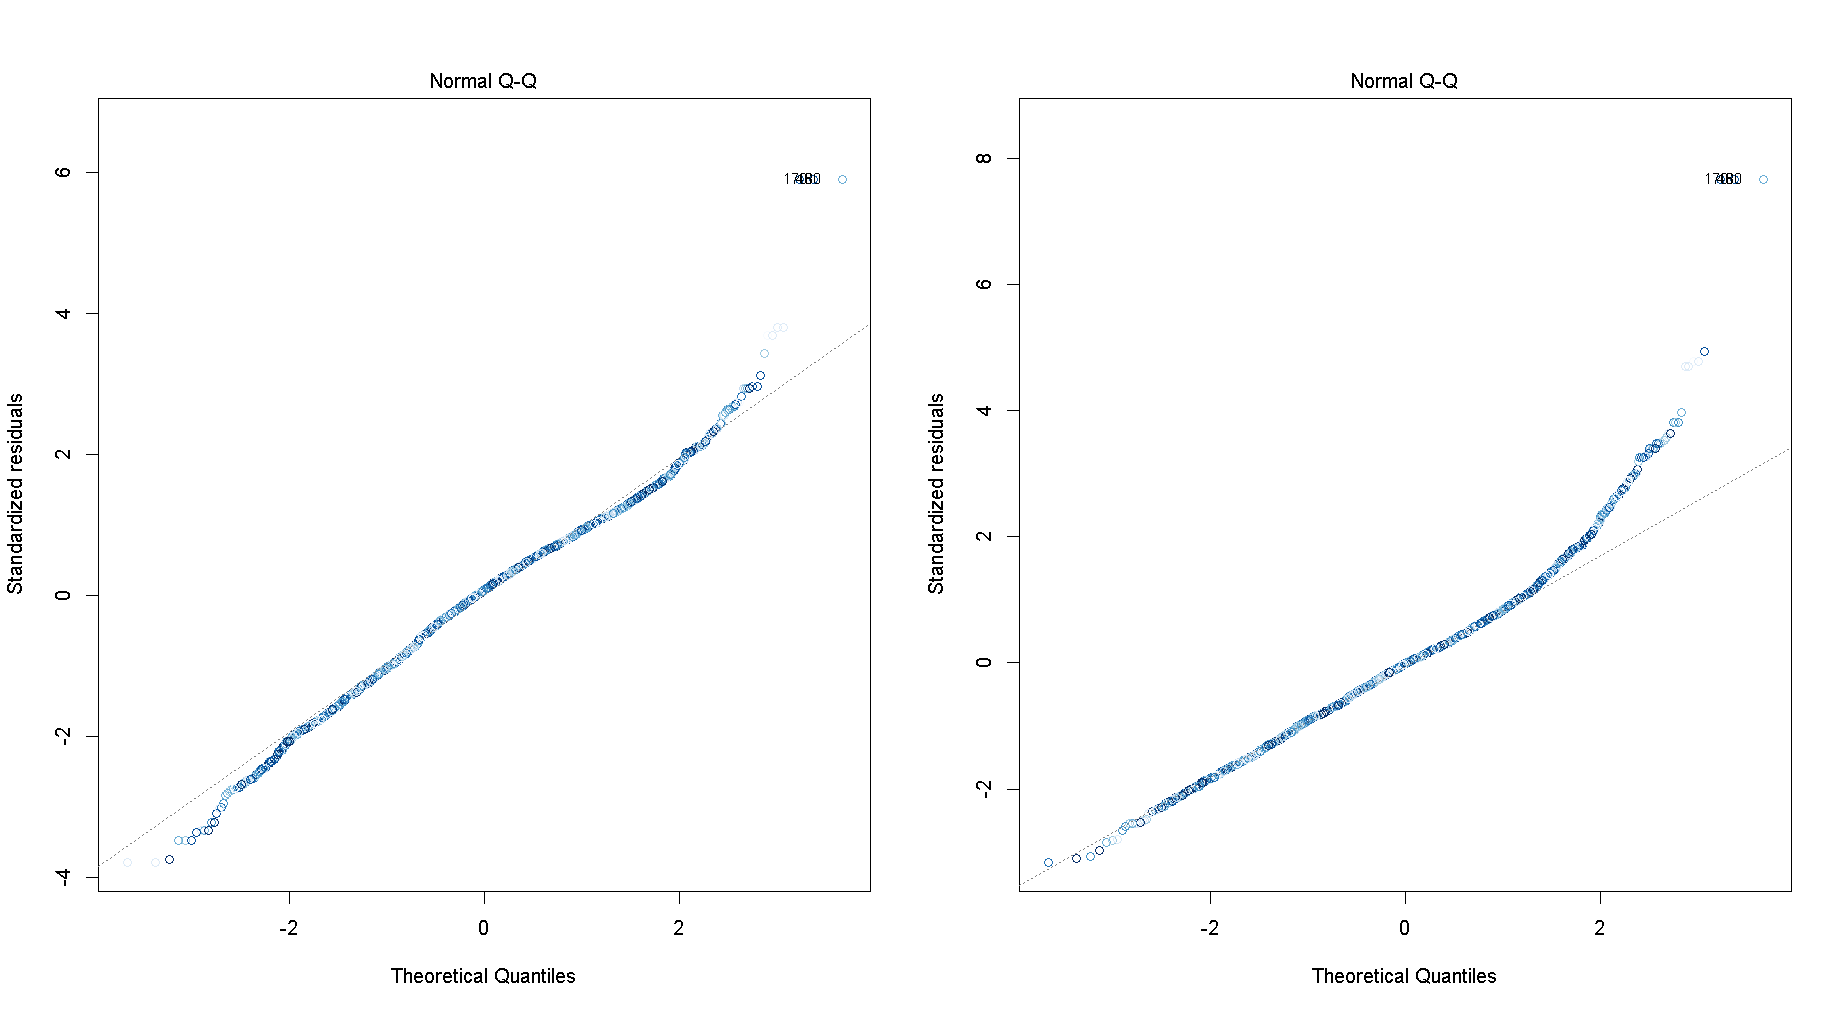
\includegraphics[width=18cm]{3.3 images/3.3.2plot.png}
    \caption{Normal Q-Q plots of residuals}
    \label{fig:qq}
\end{figure}

\subsubsection{Scale-location plot and assumption of equal variance}
 The standardized residual is given by $\frac{y_i-\hat y_i}{\sqrt{\hat y_i}}$
The standardized residual is a measure of the strength of the difference between observed and expected values. 

A scatter plot showing the square root of the absolute value of standardised residuals against fitted values is known as a scale-location plot.
This graph indicates if residuals are distributed evenly across predictor ranges.
This is how we may graphically test the equal variance assumption. If the graph is spread equally across the horizontal line, the assumption is meaningful and it is so in our linear model:

%Two Figures 

\begin{figure}[H]
    \centering
    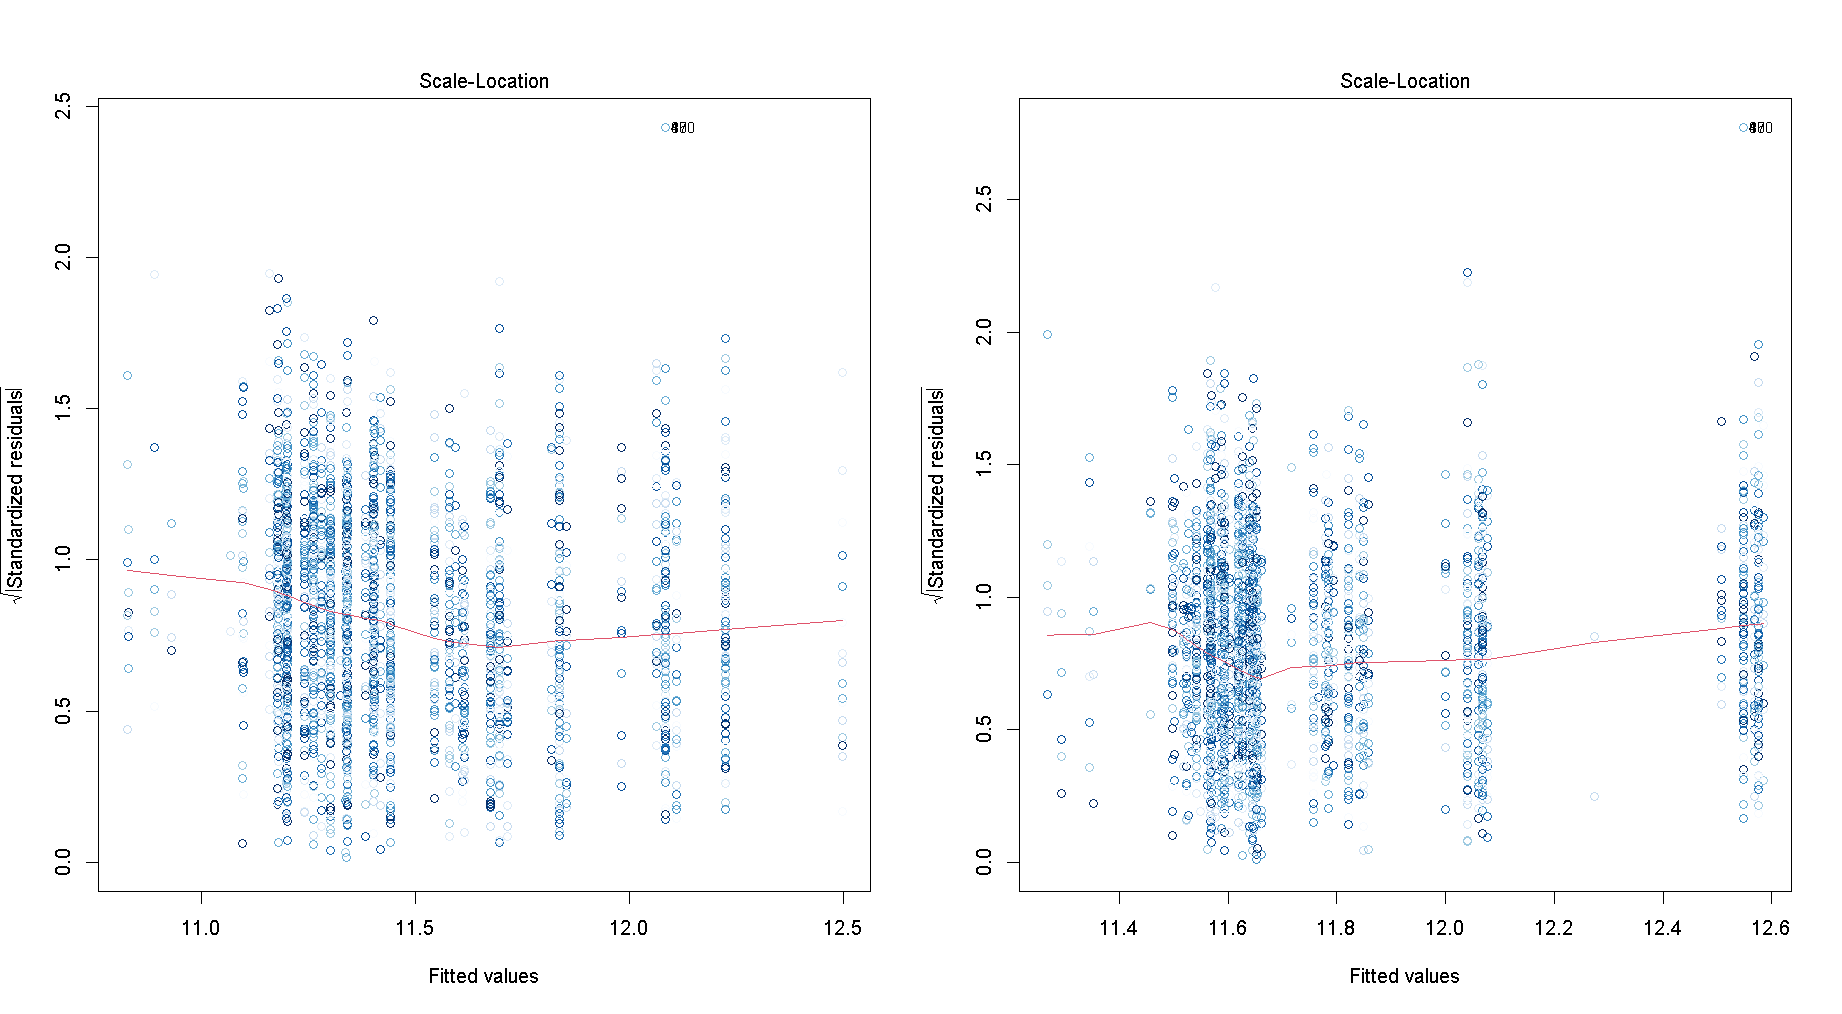
\includegraphics[width=18cm]{3.3 images/3.3.3plot.png}
    \caption{Scale Location plot}
    \label{fig:scale}
\end{figure}

All the plots above show that the hedonic pricing model with \acrshort{ols} is indeed a good way to model the dependence of prices and locational, energy factors.

\subsubsection{Leverage}
The leverage score for the $i^{th}$ independent observation $x_i$ is given as:
$$h_{ii}=[H]_{ii}=\textbf{x}_i^T(X^TX)^{-1}\textbf{x}_i=h_{ii}=\frac{\partial \hat y_i}{\partial y_i}$$
It is the degree by which $i$th measured value influences the $i$th fitted value (i.e., $\hat y_i$)
Points with extreme values of variables $x_i$ are said to have high leverage. High leverage points have a stronger capacity to shift the regression line and can be influential, causing the outcome and accuracy to be distorted.

\begin{figure}[H]
    \centering
    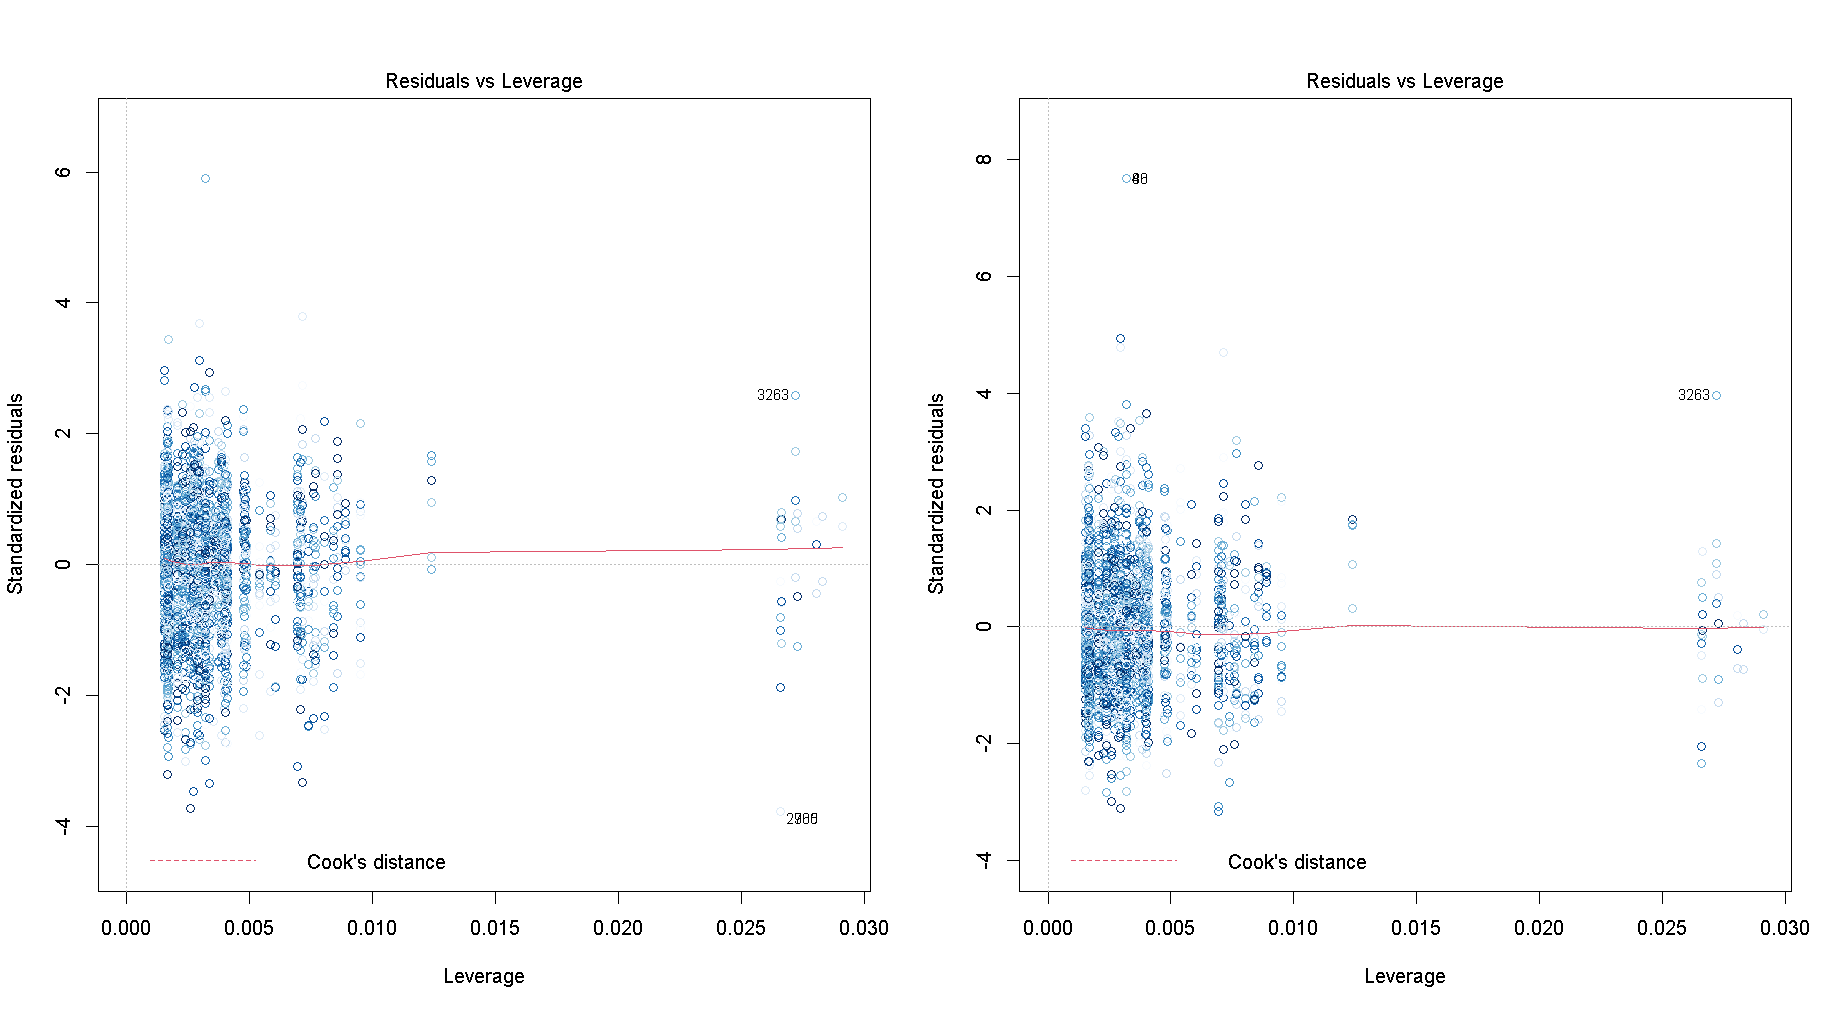
\includegraphics[width=18cm]{3.3 images/3.3.4.png}
    \caption{Standarized Residuals vs Leverage}
    \label{fig:lev}
\end{figure}

\autoref{fig:lev} below shows the standarized residuals plotted against the leverage. The contour lines of Cook's Distance are not visible in the graph. Hence, it is evident that the number of outliers are too less. So, we do not need to rerun the model by removing outliers.

\subsubsection{Cook's Distance}
Data points with large residuals (outliers) and/or high leverage may distort the outcome and accuracy of a regression.
The Cook’s distance statistic for every observation measures the extent of change in model estimates when that particular observation is omitted. 
Cook's distance $D_{i}$ of observation $i$ is defined as the sum of all the changes in the regression model when observation $i$ is removed from it
$$D_{i}={\frac {1}{(K+1)s^{2}} \sum_ {j=1}^{n}(\hat y_j-\hat y_{j(i)})}={\frac {e_{i}^{2}}{(K+1)s^{2}}}\left[{\frac {h_{ii}}{(1-h_{ii})^{2}}}\right].$$
where ${\widehat {y\, }}_{j(i)}$ is the fitted response value obtained when excluding $i$, and $s$ is the standard error.
\autoref{fig:cooks1} shows the Cook's Distance of each response value.Hence, we can notice that the Cook's Distance is mostly small for each value.
\begin{figure}[H]
    \centering
    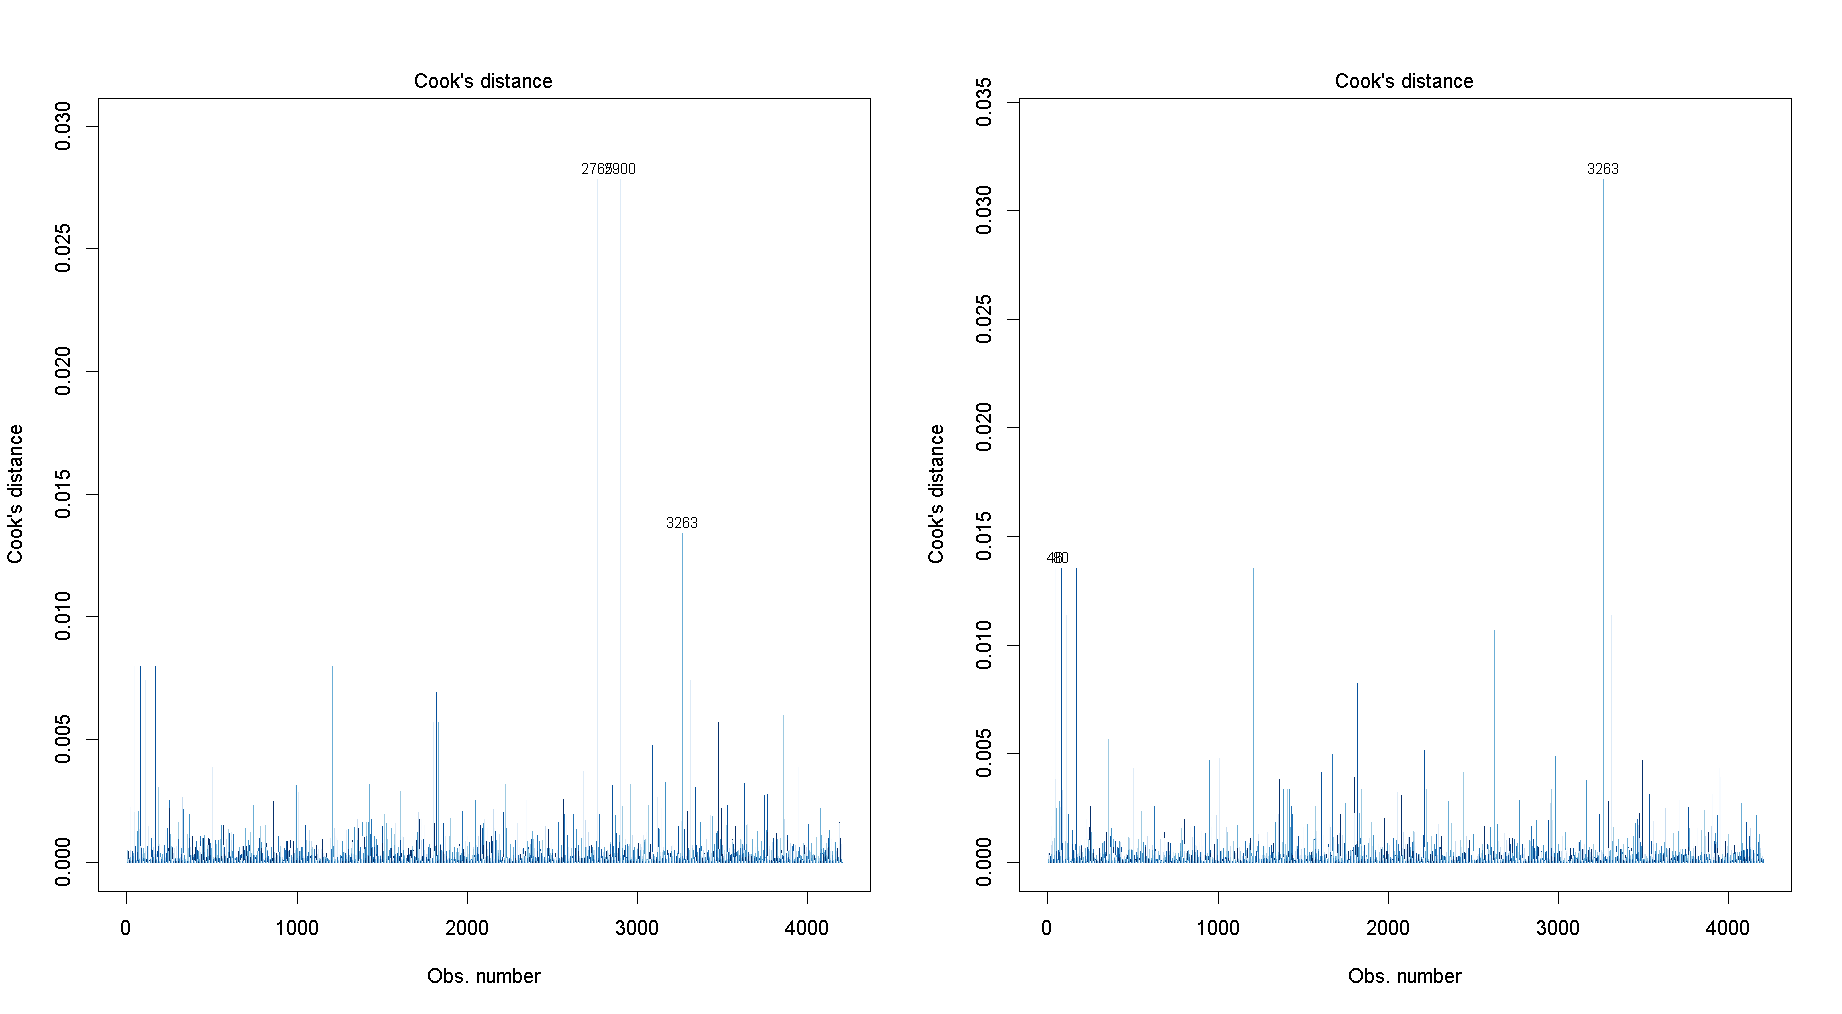
\includegraphics[width=18cm]{3.3 images/3.3.4.2.png}
    \caption{Cook's Distance plotted against row number}
    \label{fig:cooks1}
\end{figure}

Hence, our fitted model is not highly distorted. We can see there are too less points with high Cook’s Distance. This shows that although the data had many outliers pointed out by the boxplot but they mostly have low influence.
\begin{figure}[H]
    \centering
    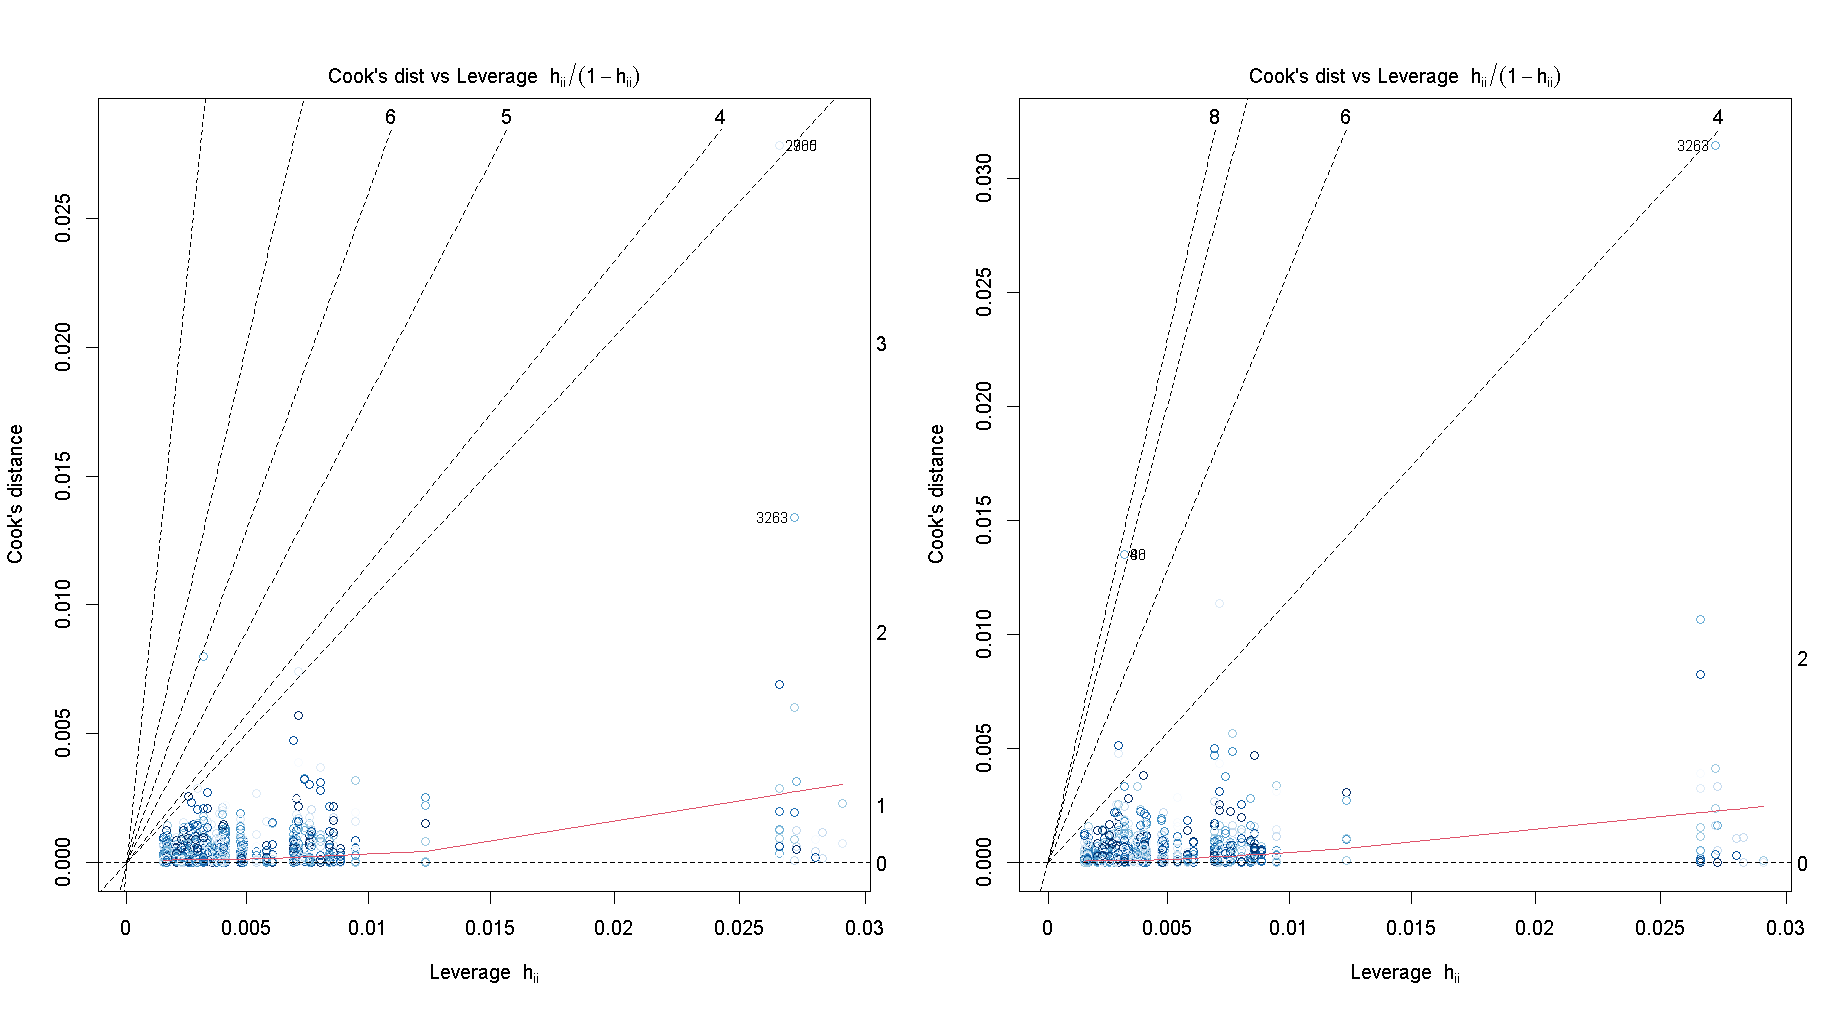
\includegraphics[width=18cm]{3.3 images/3.3.4.1.png}
    \caption{Cook's Distance plotted against Leverage.The contours in the scatterplot are standardized residuals labelled with their magnitudes}
    \label{fig:cooks2}
\end{figure}
On the other hand \autoref{fig:cooks2} shows the plot of leverage and cooks distance.

\section{Price vs socio-economic variables}
We would like to relate \gls{price1} and \gls{price2} with the socio-economic variables \gls{imdg}, \gls{income}, \gls{emp}, \gls{educ}, \gls{health}, \gls{crime}, \gls{barrier}, \gls{living}. This would reveal the dependency of housing prices on socio-economic environment.
In many statistical techniques, we assume that the errors are normally distributed and regression is one of them. The plots given below clearly show that the \gls{price1} and \gls{price2} variables are not normal.

\begin{figure}[H]
    \centering
    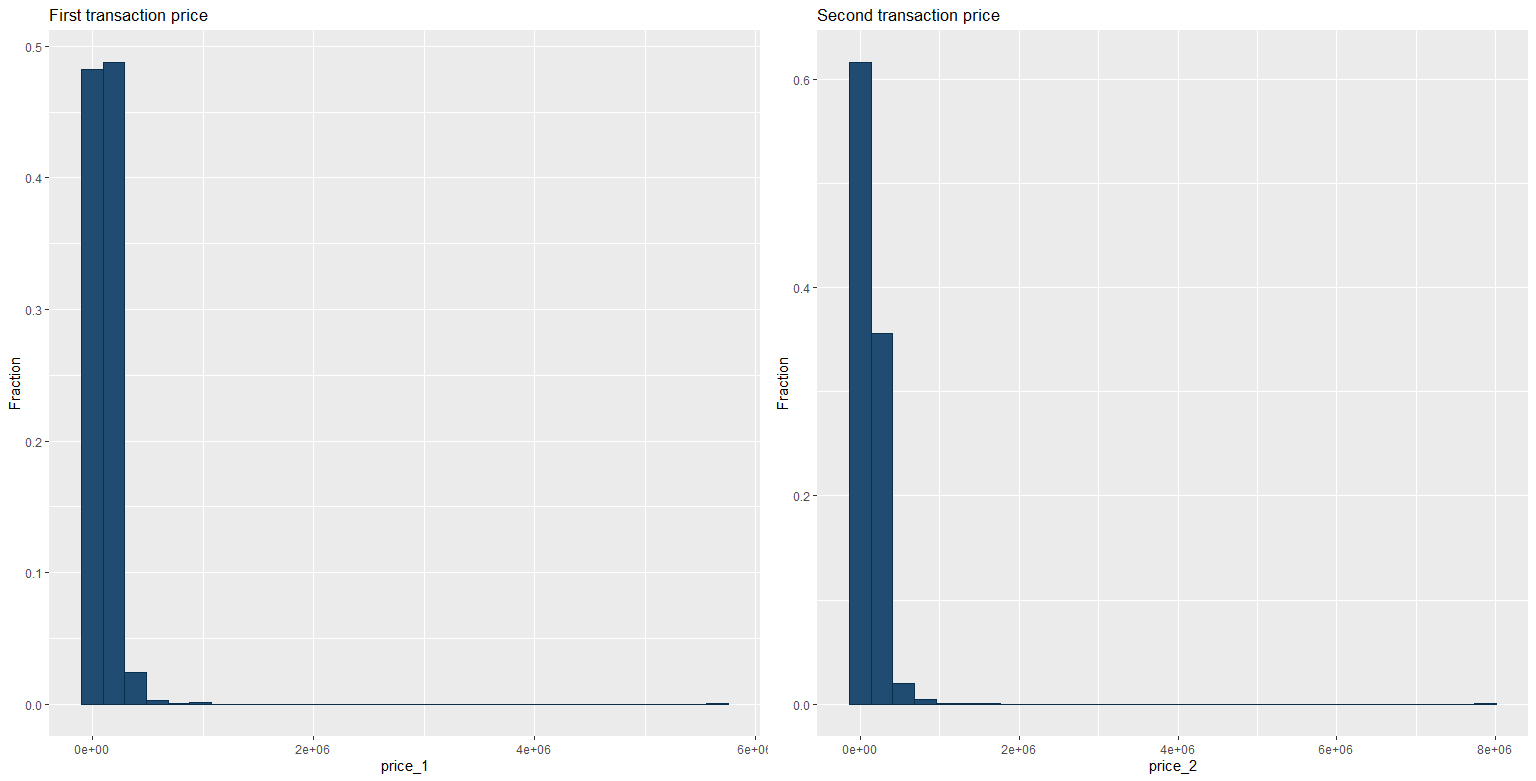
\includegraphics[width=18cm]{4. price vs socio-eco images/4non-normalplots.png}
    \caption{Distributions of the price paid in the first (left hand side) and second (right hand side) property sale transactions}
    \label{fig:prices}
\end{figure}

Instead of directly applying linear regression, we start by applying box-cox transformation on the dependent variable, developed by Box and Cox(1964).

\subsection{Box-cox transformation}
\label{boxcox}
The Box-Cox transformation transforms our data so that it closely resembles a normal distribution. Suppose variable $y$ is regressed against variable $x$. The linear model is a very good fit if $y$ is normally distributed. One reason is that confidence intervals and hypothesis tests are all based on this assumption. The objective of box-cox transformation is to transform $y$ to $y^{(\lambda)}$ so that transformed $y$ is approximately normal. The family of transformations considered are:
$$  y^{(\lambda)}=\left\{\begin{array}{ll}
      \frac{y^{\lambda}-1}{\lambda} & \lambda\neq 0 \\
      \ln (y) & \lambda=0 \\
\end{array} \right.$$
By using maximum likelihood estimator, a value of $\lambda$ is found which makes $y^{(\lambda)}$ approximately normal.

\subsection{Results}
R already has a function in its MASS library, \textbf{boxcox(object, …)} where object refers to the linear model we want to fit. After running the code, it is noticed that, 
$$\lambda_{\textrm{\gls{price1}}}=0.02$$
$$\lambda_{\textrm{\gls{price2}}}=-0.3$$
We take $0.02 \approx 0$, and we transform \gls{price1} variable to $\ln(\textrm{\gls{price1})}$ and \gls{price2} variable to $\frac{(\textrm{\gls{price2}})^{-0.03}-1}{-0.03}$.\\

\begin{figure}[H]
    \centering
    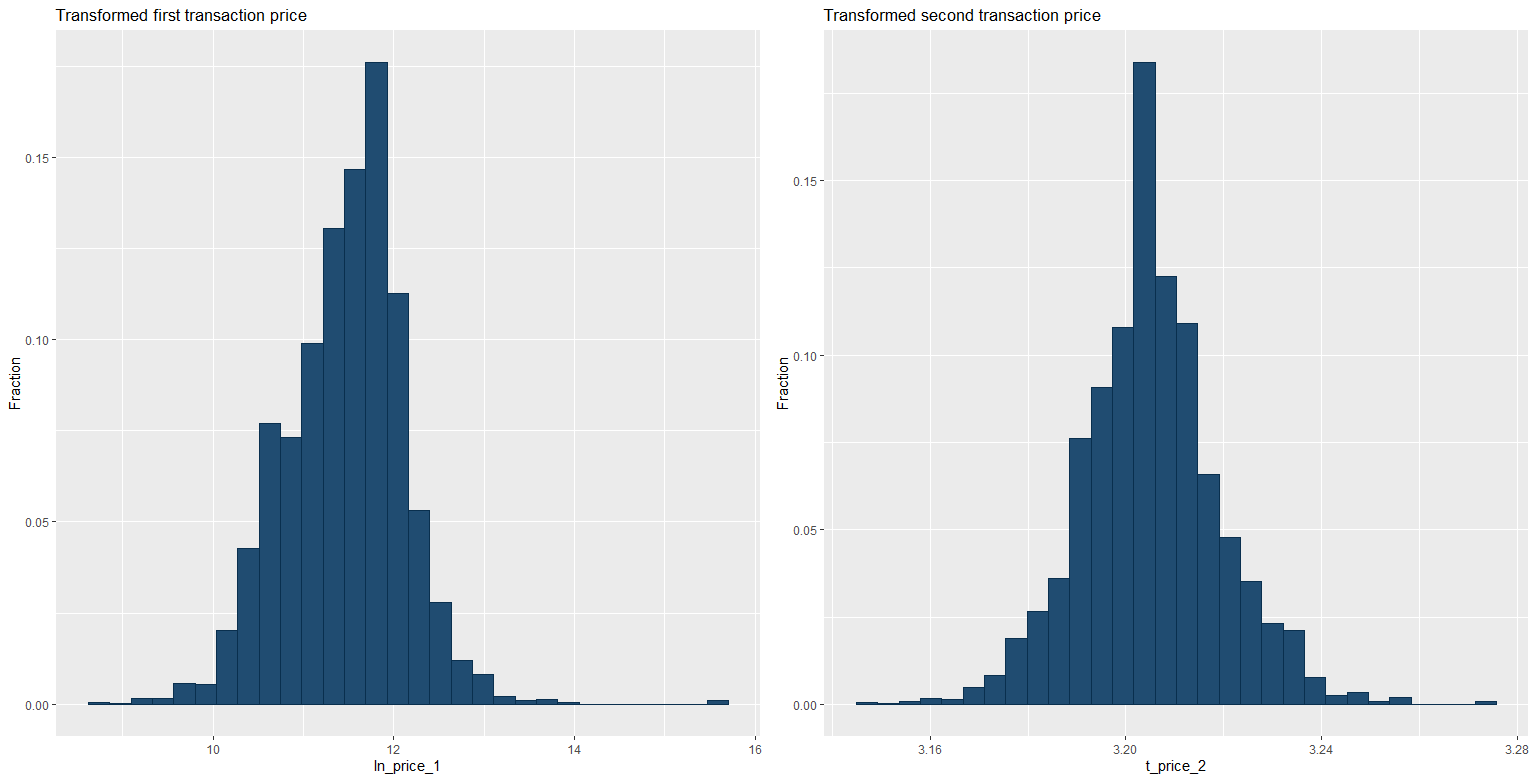
\includegraphics[width=18cm]{4. price vs socio-eco images/4t_normalplots.png}
    \caption{Distributions of the transformed price paid in the first (left hand side) and second (right hand side) property sale transactions}
    \label{fig:t_prices}
\end{figure}
The plots above are symmetric and look like normal distribution. We can now move to regression analysis.
\footnote{\textbf{Note}: The \autoref{fig:corrmat} shows the pairwise correlation in the various socio-economic variables. This may result into multicollinearity in our model. Although, the coefficient s and p-values are affected by multicollinearity, but the forecasts, precision of the predictions, and goodness-of-fit statistics are unaffected. Our primary purpose is to generate predictions and hence we are not addressing multicollinearity.}
\subsection{Summary}

\begin{table}[H]
\centering
\begin{tabular}{c c c c c c} 
 \hline
 Variable & Estimate & Std Error & t-value & Pr($>|t|$) &   \\ [0.5ex] 
 \hline
 (Intercept) & 10.82817670995 & 0.04523532930 & 239.374 & 0(approx) & *** \\
 imd\_score & -0.00006253022 & 0.00000696566 & -8.977 & 0(approx) & *** \\
 income\_score & -0.00001487051 & 0.00000390421 & -3.809 & 0.000142 & *** \\
 emp\_score & 0.00003609509 & 0.00000368207 & 9.803 & 0(approx) & *** \\
 educ\_score & 0.00003438949 & 0.00000196613 & 17.491 & 0(approx) & *** \\
 health\_score & 0.00003242077 & 0.00000250168 & 12.960 & 0(approx) & *** \\
 crime\_score & 0.00000174045 & 0.00000167774 & 1.037 & 0.299622 &  \\
 barrier\_score & -0.00000001551 & 0.00000146222 & -0.011 & 0.991539 &  \\  
 living\_score & 0.00001157480 & 0.00000167902 & 6.894 & 0(approx) & *** \\ [1ex]
 \hline
\end{tabular}
\captionsetup{justification=centering}  
\caption{Trasformed \gls{price1} vs socio-economic variables.\\ Signif. codes:  0 `***' 0.001 `**' 0.01 `*' 0.05 `.' 0.1 ` ' 1}
\label{table:3}
\end{table}

\begin{table}[H]
\centering
\begin{tabular}{c c c c c c} 
 \hline
 Variable & Estimate & Std Error & t-value & Pr($>|t|$) &  \\ [0.5ex] 
 \hline
 (Intercept) & 3.18665988102 & 0.00087845134 & 3627.588 & 0(approx) & *** \\
 imd\_score & -0.00000193203 & 0.00000013527 & -14.283 & 0(approx) & *** \\
 income\_score & -0.00000017160 & 0.00000007582 & -2.263 & 0.0237 & * \\ 
 emp\_score & 0.00000103479 & 0.00000007150 & 14.472 & 0(approx) & *** \\
 educ\_score & 0.00000088244 & 0.00000003818 & 23.112 & 0(approx) & *** \\
 health\_score & 0.00000085907 & 0.00000004858 & 17.683 & 0(approx) & *** \\
 crime\_score & 0.00000014584 & 0.00000003258 & 4.476 & 0.000008 & *** \\
 barrier\_score & 0.00000004633 & 0.00000002840 & 1.632 & 0.1028 &  \\  
 living\_score & 0.00000026311 & 0.00000003261 & 8.069 & 0(approx) & *** \\ [1ex]
 \hline
\end{tabular}
\captionsetup{justification=centering}
\caption{Trasformed \gls{price2} vs socio-economic variables.\\Signif. codes:  0 `***' 0.001 `**' 0.01 `*' 0.05 `.' 0.1 ` ' 1}
\label{table:4}
\end{table}


\subsection{Partial residue plots}
\label{prp}
A partial residual plot is a scatterplot to show the relationship between a given independent variable($x_i$) and the response variable($y$) given that other independent variables are also in the model.
The partial residual plot is a useful tool to verify if there exists any linear relationship of a given variable on the response variable.
Partial residuals are computed as:
$$\textrm{Residuals} +{\hat {\beta }}_{i}x_{i}$$
Note that the Residuals are the residuals from the full model.\\
In partial residual plot, these partial residuals are plotted against $x_i$. The termplot function of R helps us to create such plots.
This function also takes the projection of the regression hyperplane to the $x_i$ vs $y$ plane. The slope of the line is the coefficient of $x_i$ in the original linear model.
Moreover, it further adds a smooth curve to the plot. This helps us analyse whether there is any non-linear relationship with the $x_i$.
\\
\begin{figure}[H]
    \centering
    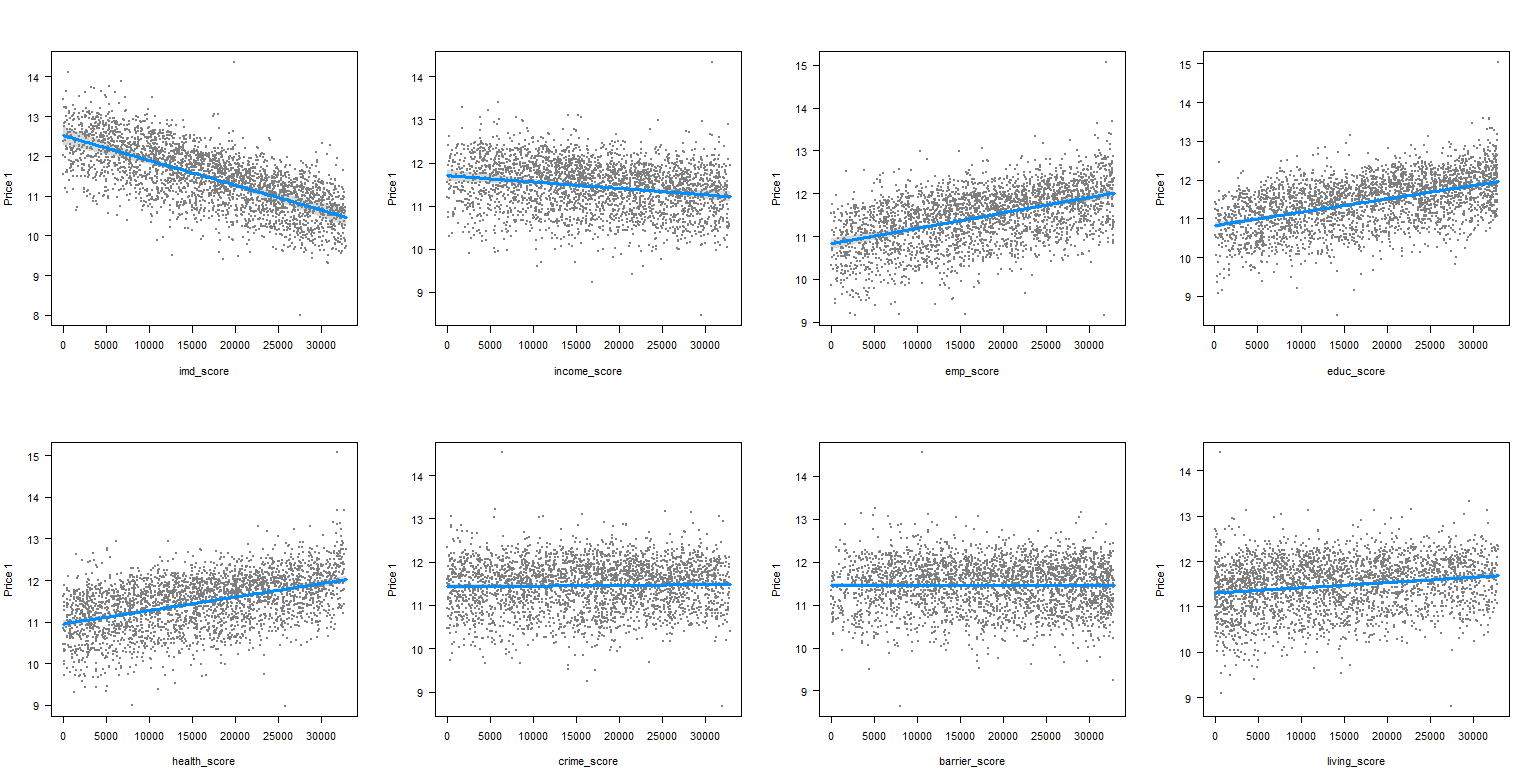
\includegraphics[width=18cm]{4. price vs socio-eco images/par.resid_1Plot.png}
    \caption{Plot of partial residuals and regression terms of transformed \gls{price1} across the predictor variables along with smooth fitted curve}
    \label{fig:prp1}
\end{figure}
\begin{figure}[H]
    \centering
    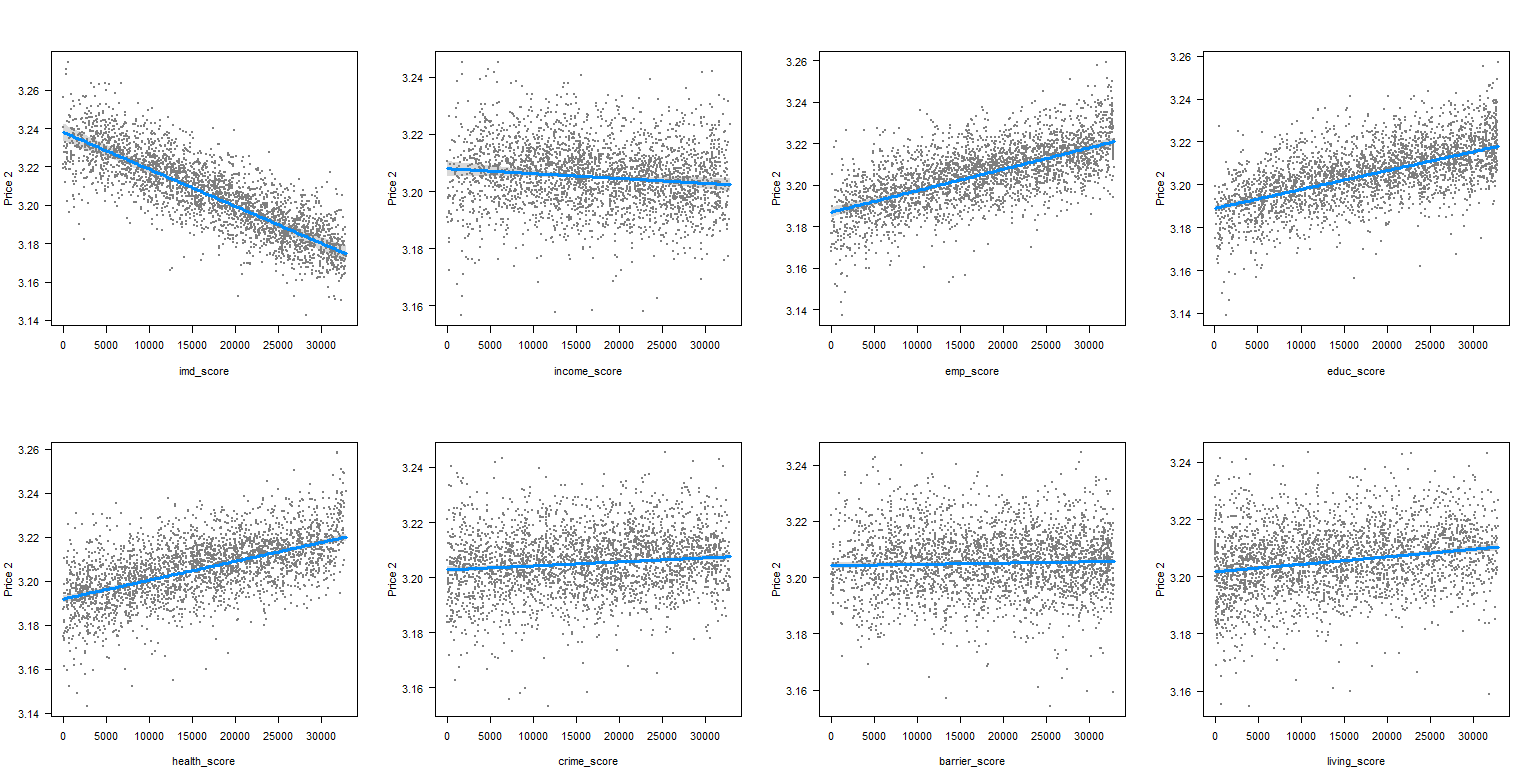
\includegraphics[width=18cm]{4. price vs socio-eco images/par.resid_2Plot.png}
    \caption{Plot of partial residuals and regression terms of transformed \gls{price2} across the predictor variables along with smooth fitted curve}
    \label{fig:prp2}
\end{figure}


The above plots suggests that there is no non-linear relationship and our model quite efficiently measures the relationship.

\section{Repeat sales index}
\label{rsi}
In this section we use the repeat-sales method to examine how house values fluctuate over time by comparing the sale prices of the same piece of property.
Using this method, assuming a house undergoes no changes, to assess how prices change over
time, one need only look at the difference in sale prices of the same house.
\subsection{Preparing the data for repeat sales index}
The original dataset had the repeat sales prices of houses. The repeat sales transactions took place from 1995 to 2012, for this data set. We made a new dataset that consisted of variables Y1995, Y1996, ... and so on upto Y2012. For any house, these variables take value -1 if the first sales transaction took place in that year, 1 if the second sales transaction took place in that year and 0 otherwise. The variable log\_change each derived as:
\begin{center}
    log\_change $=$ ln\_price\_2 $-$ ln\_price\_1
\end{center}
\subsection{Regression}
Let there be $T$ time periods where sales can occur from $y_1, ..., y_T$. Each $y_t$ is a categorical variable: $y_t=-1$($y_t=1$ resp.) if first (second resp.) sale takes place in year $y_t$ and $y_t=0$ otherwise. Let $B_{t}'$ denote the (true, but unknown) repeat sales index for year $y_t$. Let $P_{it}$ and $P_{it'}$ denote the sales prices of $i$th house at the $t$th period. A probabilistic model is made as follows:
$$\frac{P_{it'}}{P_{it}}=\frac{B_{t'}}{B_{t}}U_{itt'}$$
Taking logarithm, 
$$\ln(P_{it'})-\ln(P_{it})=\ln(B_{t'})-\ln(B_{t})+u_{itt'} $$
where $u_{itt'}=\ln(U_{itt'})$ is the residual. Again, four assumptions on the distribution of the residuals: They have mean 0, constant variance, $u_{itt'}\sim N(0, \sigma^2)$, uncorrelated with each other.  The above equation can be written as:
$$\ln(P_{it'})-\ln(P_{it})=\sum_{j=1} ^{T}{y_j \ln(B_{j})} +u_{itt'} $$


The model in the above equation is fit using linear regression and the estimated log indices are transformed to repeat sales indices with the exponential function. The estimated linear equation will be:
$$\ln (\hat P_{t'})-\ln(\hat P_t)=\hat B_{0}+\sum_{j=1} ^{l} \ln (\hat B_j) y_{j}$$
\\
We run \acrshort{ols} regression using R where the dependent variable is log\_change and the regressors are Y1995, Y1996, ..., Y2012 (called $y_1, ..., y_T$, $T=18$). The Y1995 is taken as base year and is held out of the regression.
 
\begin{figure}[H]
    \centering
    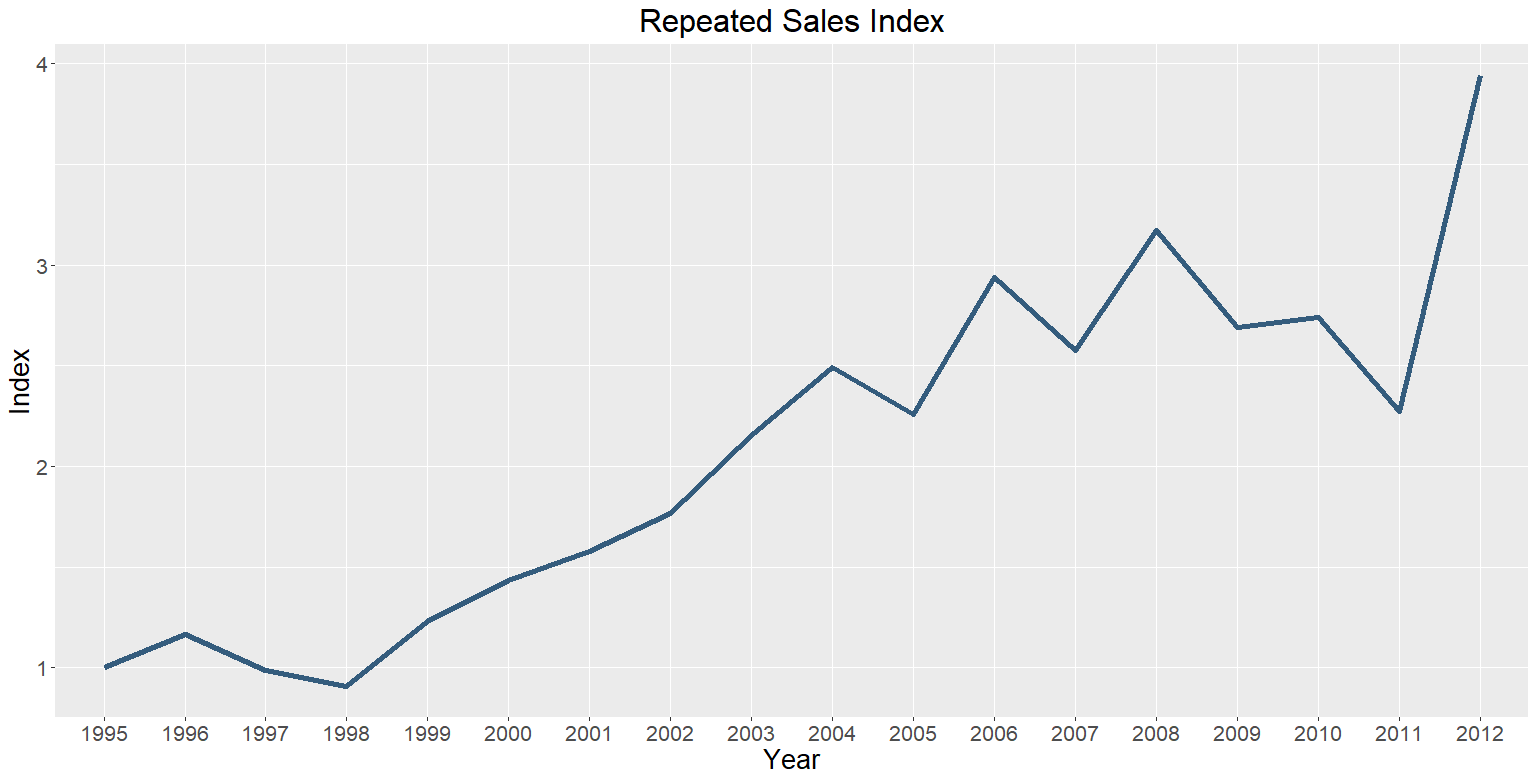
\includegraphics[width=18cm]{5. RSI images/rsiplot.png}
    \caption{Repeat Sales Index of each year with base year being 1995}
    \label{fig:rsi}
\end{figure}

The \autoref{fig:rsi} shows the line graph of the estimated coefficients. There is increase of change in prices over years. The inflation is prices is evident the figure. There are major retractions in 1998, 2011. The index reaches its maximum at 2012.

\section{Conclusions}
\label{sec:conc}
Landlords can make informed investments when there is a clear link between price and energy efficiency. In addition, we have taken regional aspects into account. We linked the pricing to socio-economic parameters in the second model. The empirical findings confirm that energy efficiency characteristics have a minor but considerable impact on both transaction prices. Furthermore, the current study was unable to control the correlation between factors. Moreover, our model was only focused on pricing, and we were unable to establish a link between \acrshort{epc}s and Regions. In order to produce a comprehensive idea on this divided incentive dilemma, the data can also be enlarged to a much larger database.

\subsection{Limitations}
\begin{itemize}
    \item For hedonic regression, a large  data must be collected and processed with. However, the data that was utilised only had 4201 values. The Hedonic Price Index calculates how much individuals are prepared to pay for alleged differences in environmental quality and its implications. However, if individuals are ignorant of the link between environmental attributes and property worth, the value will not be reflected in the price. 
    \item One major issue is that repeat sales approach remove residences that sell only once during the data gathering period. Another issue is that all houses age, and as a result, the houses alter, which might impact the index, which is not taken into account here.
    \item While using box-cox transformation, the lambda obtained for \gls{price2} was not zero, and is therefore not possible to interpret. Also box-cox transformation does not always guarantee normality.
\end{itemize}
\subsection{Extensions}
The chief findings support existing literature on “Is there an Economic Case for Energy-Efficient Dwellings in the UK Private Rental Market?” in the housing market by adding to empirical evidence on the relationship between energy efficiency ratings and pricing decisions and demonstrating that the features captured by \acrshort{epc}s are widely significant to housing price.

Here is the list of extension we have attempted, which were not there in the original paper.
\begin{enumerate}
    \item Plots for visualization viz.
    \begin{itemize}
        \item \autoref{fig:corrmat}
        \item \autoref{fig:mprice}
        \item \autoref{fig:boxprice}
        \item \autoref{fig:hedonic}
    \end{itemize}
    \item Diagnostic plots in \autoref{diag_plot}
    \item Box-Cox transformation in \autoref{boxcox}
    \item Partial Residue Plots, \autoref{prp}
    \item Repeat sales index of the the price variables across years, \autoref{rsi}
\end{enumerate}

\subsection{Future Scope}
More complex regressions can be applied in terms of statistical approaches. The correlation between components could not be controlled in the current investigation. The \autoref{fig:corrmat} clearly demonstrates that several factors that we expected to be independent have a significant degree of correlation. Case and Quigley's (1991) hybrid index can also be used.
The Case-Shiller(1987, 1989) regression method can be used to make a development on the repeat sales index. A recent method called autoregressive index has been developed by Nagaraja, Brown, and Zhao (2011).
On a bigger dataset, the analysis may be run with additional variables, taking into account, housing attributes.etc.
\section{References}
\begin{enumerate}
    \item Franz Fuerst, Michel Ferreira Cardia Haddad(2020). \href{https://doi.org/10.1016/j.dib.2020.106359}{``Real estate data to analyse the relationship between property prices, sustainability levels and socio-economic indicators."} Data in Brief. 33 106359.
    \item F. Fuerst, M.F.C. Haddad, H. Adan(2015). \href{https://doi.org/10.1016/j.jclepro.2019.118642}{``Is there an economic case for energy-efficient dwellings in the UK private rental market?"} Journal for Cleaner Prod. 245 (2020) 118642. 
    \item F. Fuerst , P. McAllister , A. Nanda , P. Wyatt(2015). \href{https://doi.org/10.1016/j.eneco.2014.12.012}{``Does  energy efficiency matter to home-buyers? an investigation of \acrshort{epc} ratings and transaction prices in England?"} Energy Economy. 48 145–156 .
    \item Bailey, M.J., Muth, R.F., Nourse, H.O. (1963). ``A regression method for real estate price index construction. Journal of the American Statistical Association." 58 933-942
    \item Ryan, Thomas P (2015). Modern Regression Methods. Wiley-Interscience.
    \item G. E. P. Box and D. R. Cox(1964). \href{https://www.jstor.org/stable/2984418}{``An Analysis of Transformations."} Journal of the Royal Statistical Society. Series B Vol. 26. No. 2.
    \item Case, K.E., Shiller, R.J. (1987). Prices of single-family homes since 1970: new indexes for four cities. New England Economic Review. Sept./Oct. 45-56. 
    \item Case, K.E., Shiller, R.J. (1989). The efficiency of the market for single family homes. The American Economic Review. 79 125-137
    \item Case, B., Quigley, J.M. (1991). The dynamics of real estate prices. The Review of Economics and Statistics. 73 50-58
    \item Chaitra H. Nagaraja. Lawrence D. Brown. Linda H. Zhao(2011). \href{https://doi.org/10.1214/10-AOAS380}{``An autoregressive approach to house price modeling."} Ann. Appl. Stat. 5 (1) 124 - 149, March 2011.
    \item \href{https://www.jstor.org/stable/24885063}{Repeat Sales House Price Index Methodology}. Journal of Real Estate Literature. Vol. 22, No. 1 (2014), pp. 23-46.
\end{enumerate}

\printglossary[type=\acronymtype]

\printglossary

\end{document}